% Options for packages loaded elsewhere
\PassOptionsToPackage{unicode}{hyperref}
\PassOptionsToPackage{hyphens}{url}
\PassOptionsToPackage{dvipsnames,svgnames,x11names}{xcolor}
\documentclass[
  11pt,
]{article}
\usepackage{xcolor}
\usepackage[margin=1in]{geometry}
\usepackage{amsmath,amssymb}
\setcounter{secnumdepth}{-\maxdimen} % remove section numbering
\usepackage{iftex}
\ifPDFTeX
  \usepackage[T1]{fontenc}
  \usepackage[utf8]{inputenc}
  \usepackage{textcomp} % provide euro and other symbols
\else % if luatex or xetex
  \usepackage{unicode-math} % this also loads fontspec
  \defaultfontfeatures{Scale=MatchLowercase}
  \defaultfontfeatures[\rmfamily]{Ligatures=TeX,Scale=1}
\fi
\usepackage{lmodern}
\ifPDFTeX\else
  % xetex/luatex font selection
\fi
% Use upquote if available, for straight quotes in verbatim environments
\IfFileExists{upquote.sty}{\usepackage{upquote}}{}
\IfFileExists{microtype.sty}{% use microtype if available
  \usepackage[]{microtype}
  \UseMicrotypeSet[protrusion]{basicmath} % disable protrusion for tt fonts
}{}
\makeatletter
\@ifundefined{KOMAClassName}{% if non-KOMA class
  \IfFileExists{parskip.sty}{%
    \usepackage{parskip}
  }{% else
    \setlength{\parindent}{0pt}
    \setlength{\parskip}{6pt plus 2pt minus 1pt}}
}{% if KOMA class
  \KOMAoptions{parskip=half}}
\makeatother
\usepackage{longtable,booktabs,array}
\usepackage{caption}
\newcounter{none} % for unnumbered tables
\usepackage{calc} % for calculating minipage widths
% Correct order of tables after \paragraph or \subparagraph
\usepackage{etoolbox}
\makeatletter
\patchcmd\longtable{\par}{\if@noskipsec\mbox{}\fi\par}{}{}
\makeatother
% Allow footnotes in longtable head/foot
\IfFileExists{footnotehyper.sty}{\usepackage{footnotehyper}}{\usepackage{footnote}}
\makesavenoteenv{longtable}
\usepackage{graphicx}
\makeatletter
\newsavebox\pandoc@box
\newcommand*\pandocbounded[1]{% scales image to fit in text height/width
  \sbox\pandoc@box{#1}%
  \Gscale@div\@tempa{\textheight}{\dimexpr\ht\pandoc@box+\dp\pandoc@box\relax}%
  \Gscale@div\@tempb{\linewidth}{\wd\pandoc@box}%
  \ifdim\@tempb\p@<\@tempa\p@\let\@tempa\@tempb\fi% select the smaller of both
  \ifdim\@tempa\p@<\p@\scalebox{\@tempa}{\usebox\pandoc@box}%
  \else\usebox{\pandoc@box}%
  \fi%
}
% Set default figure placement to htbp
\def\fps@figure{htbp}
\makeatother
\setlength{\emergencystretch}{3em} % prevent overfull lines
\providecommand{\tightlist}{%
  \setlength{\itemsep}{0pt}\setlength{\parskip}{0pt}}
\usepackage[numbers]{natbib}
\bibliographystyle{unsrtnat}
\usepackage{bookmark}
\IfFileExists{xurl.sty}{\usepackage{xurl}}{} % add URL line breaks if available
\urlstyle{same}
\hypersetup{
  pdftitle={Mapping Superconductivity Research for AI: A Two-Axis Survey of 10{,}249 Preprints and Where Machine Learning Can Actually Help},
  pdfauthor={Mingguang Chen},
  colorlinks=true,
  linkcolor={Maroon},
  filecolor={Maroon},
  citecolor={Blue},
  urlcolor={Blue},
  pdfcreator={LaTeX via pandoc}}

\title{Mapping Superconductivity Research for AI: A Two-Axis Survey of
10,249 Preprints and Where Machine Learning Can Actually Help}
\author{Mingguang Chen\textsuperscript{1,$*$}\\[6pt]
{\small \textsuperscript{1}DeepGrounding}\\[2pt]
{\small \textsuperscript{$*$}Corresponding author. Email: \href{mailto:deepgroundingai@gmail.com}{deepgroundingai@gmail.com}}}
\date{7 September 2026}

\begin{document}
\maketitle
\begin{abstract}
Superconductivity research generates enormous quantities of data and has
a poor record of predicting its own discoveries, which makes it an
obvious target for AI for Science and a poorly understood one. We map
the field systematically. Every arXiv preprint filed under
cond-mat.supr-con between September 2021 and September 2026 was
harvested month by month, giving 10,303 records, of which 10,049 survive
off-topic filtering at a measured bleed rate of 2.5\%; a targeted
supplement adds 200 on-topic records on AI for materials. Each record is
classified along two axes -- material family and mode of inquiry -- by a
language-model pass validated against hand labels at 85.6\% and 88.4\%
agreement, with per-class recall reported. We then assess each cell of
the resulting grid for data availability, benchmark maturity and
validation cost. Three findings emerge. Machine learning has barely
entered the field: 1.2\% of the systematic corpus uses an AI method in
its own work. Adoption tracks validation cost rather than data volume or
scientific stakes, concentrating in ab initio screening and neural
quantum states, where a calculation can check a prediction, and in
device metrology, where instruments generate their own labels. And
synthesis, which Section 3 finds to be the rate-limiting step across
material families, contains a single AI-tagged paper. The gap between
prediction and measurement is concrete: recent screens advertise
candidates above 200 K, while the one closed
prediction-synthesis-measurement loop in the recent literature delivered
superconductors between 2.5 and 6.5 K. We conclude that the
highest-value interventions are releasing labelled characterization
data, building a time-stamped benchmark of experimentally confirmed
superconductors, and modelling synthesizability rather than automating
synthesis. Corpus, labels and scripts are released.
\end{abstract}

\section{Introduction}\label{introduction}

Superconductivity is an unusually well-instrumented field with an
unusually poor prediction record. A century after Onnes, the mechanism
of the highest-\(T_c\) families is still contested, the compounds that
matter were mostly found by chemical intuition and persistence, and two
of the most prominent recent claims of room-temperature
superconductivity have been retracted. It is exactly the sort of field
that AI-for-Science rhetoric promises to transform.

Whether it can, and where, is an empirical question about the field's
structure rather than about the capability of models. A machine-learning
method needs three things: data in a form it can consume, a target
quantity worth predicting, and a way of finding out whether a prediction
was right. Different parts of superconductivity research supply these to
wildly different degrees. High-pressure hydride work has a computable
target and a mature calculation pipeline. Cuprate physics has four
decades of spectra and no agreed quantity to predict. Thin-film
synthesis has the field's real bottleneck and almost no machine-readable
record of what has been tried.

This survey makes that structure explicit. We harvest every arXiv
preprint filed under \texttt{cond-mat.supr-con} between September 2021
and September 2026, classify each along two axes -- the material family
it studies and the mode of inquiry it uses -- and then evaluate each
cell of the resulting grid for what a machine-learning method could
contribute to it. The corpus is 10,249 records after off-topic
filtering, and the classification is validated against hand labels with
the agreement rates and per-class recall reported in full.

Three results follow. \textbf{Machine learning has barely entered this
field}: 1.2\% of the systematically harvested corpus uses an AI method
in its own work. \textbf{Where it has entered, it tracks validation
cost}, clustering in the cells where a calculation can check a
prediction and in device metrology where instruments generate their own
labels, rather than in the cells with the most data or the greatest
scientific stakes. And \textbf{the field's actual bottleneck is the
emptiest cell}: synthesis, where the corpus contains a single AI-tagged
paper.

The contribution is therefore threefold: a systematically harvested and
openly released corpus of the field's recent literature; a two-axis
taxonomy that has been tested against hand labels rather than asserted;
and a per-cell assessment of AI readiness that identifies where effort
is likely to pay off and, more usefully, where current enthusiasm is
misdirected. Section 2 fixes the vocabulary, states the taxonomy,
positions the survey against existing reviews and documents the corpus.
Sections 3 and 4 walk the two axes. Section 5 reports what AI has
actually done in this field, critical literature included. Section 6
gives the readiness assessment and the resulting priorities. Section 7
asks what the emerging AI-for-science infrastructure would have to
deliver for the field's central target to come within reach, and what
would falsify that route. Section 8 offers three testable hypotheses
about why the field looks the way it does.

\section{Preliminaries and taxonomy}\label{preliminaries-and-taxonomy}

\section{Terms this field
overloads}\label{terms-this-field-overloads}

A survey that spans nine material families and five modes of work has to
fix its vocabulary first, because several of the terms below carry
different meanings in different corners of the literature.

\textbf{Critical temperature.} \(T_c\) is quoted from several
inequivalent operational definitions: the onset of a resistive drop, the
midpoint of the transition, the zero-resistance point, and the
temperature at which diamagnetic screening appears. The gap between
onset and zero resistance is small in clean conventional samples and
large in inhomogeneous ones, which is exactly where contested claims
live. Throughout this survey we say which definition a reported number
uses when the distinction bears on the claim, and we treat a resistive
onset without a magnetic signature as weaker evidence than the two
together.

\textbf{Conventional and unconventional.} We use \emph{conventional} to
mean pairing mediated by electron-phonon coupling and describable within
Migdal-Eliashberg theory \citep{bardeen1957theory}, and
\emph{unconventional} to mean a gap function that changes sign or breaks
a lattice symmetry, whatever the glue. High-pressure hydrides are
therefore conventional in mechanism while being extreme in \(T_c\), and
this survey groups them with the electron-phonon family rather than with
the cuprates they are often headlined against.

\textbf{Prediction versus discovery.} A computed structure with a
favourable calculated \(T_c\) is a prediction. A material that has been
made and measured is a discovery. Papers routinely use ``discovery'' for
the former, and the AI-for-materials literature does so more often than
the superconductivity literature does. We reserve \emph{discovery} for
the experimental sense and say \emph{predicted candidate} otherwise.
This distinction carries most of the weight in Section 5.

\textbf{AI-discovered.} We treat a material as AI-discovered only when a
machine-learning model selected or generated the candidate, the material
was subsequently synthesised, and superconductivity was measured. Weaker
uses of the phrase -- a screen that ranked a known compound highly, or a
model that reproduced a \(T_c\) after the fact -- are described as such.

\section{The two axes}\label{the-two-axes}

The taxonomy has two axes plus a lens (Figure 1).

\textbf{Axis 1, material family}, is what the paper is about:
\texttt{conv} (conventional and electron-phonon systems, including
high-pressure hydrides), \texttt{cuprate}, \texttt{febased},
\texttt{nickelate}, \texttt{unconv\_other} (heavy fermion, ruthenate,
organic, noncentrosymmetric bulk systems), \texttt{lowd}
(two-dimensional, interface, moiré and kagome systems), \texttt{topo}
(topological superconductivity and Majorana platforms), \texttt{device}
(qubits, detectors, magnets, cables, circuits), and \texttt{general}
(material-agnostic theory, formalism and instrumentation).

\textbf{Axis 2, mode of inquiry}, is how the work was done:
\texttt{theory}, \texttt{abinitio}, \texttt{discovery},
\texttt{synthesis}, \texttt{characterization}. This axis deliberately
does not encode whether a topic is applied. An earlier version of this
taxonomy carried a sixth value, \texttt{application}, and it failed a
measurement: it mixed \emph{how} the work was done with \emph{what it
was for}, and characterization-versus-application was the single largest
source of disagreement both for keyword rules and for two independently
benchmarked language models. Application context is carried by the
\texttt{device} family instead, so a qubit paper is labelled theory,
synthesis or characterization like any other paper.

\textbf{The AI lens} applies only to papers that use a machine-learning
method in their own work: \texttt{surrogate} (regression and
classification models, symbolic regression), \texttt{gnn\_potential}
(graph networks and machine-learned interatomic potentials),
\texttt{generative} (diffusion, VAE, flow models for structures and
compositions), \texttt{llm} (language models, agents, literature
mining), \texttt{nqs} (neural quantum states), and
\texttt{autonomous\_exp} (self-driving laboratories, closed-loop active
learning).

The axes are the contribution of this survey, and Sections 3 through 5
are organised along them. Section 6 evaluates each cell for what AI can
currently do in it.

\begin{figure}
\centering
\pandocbounded{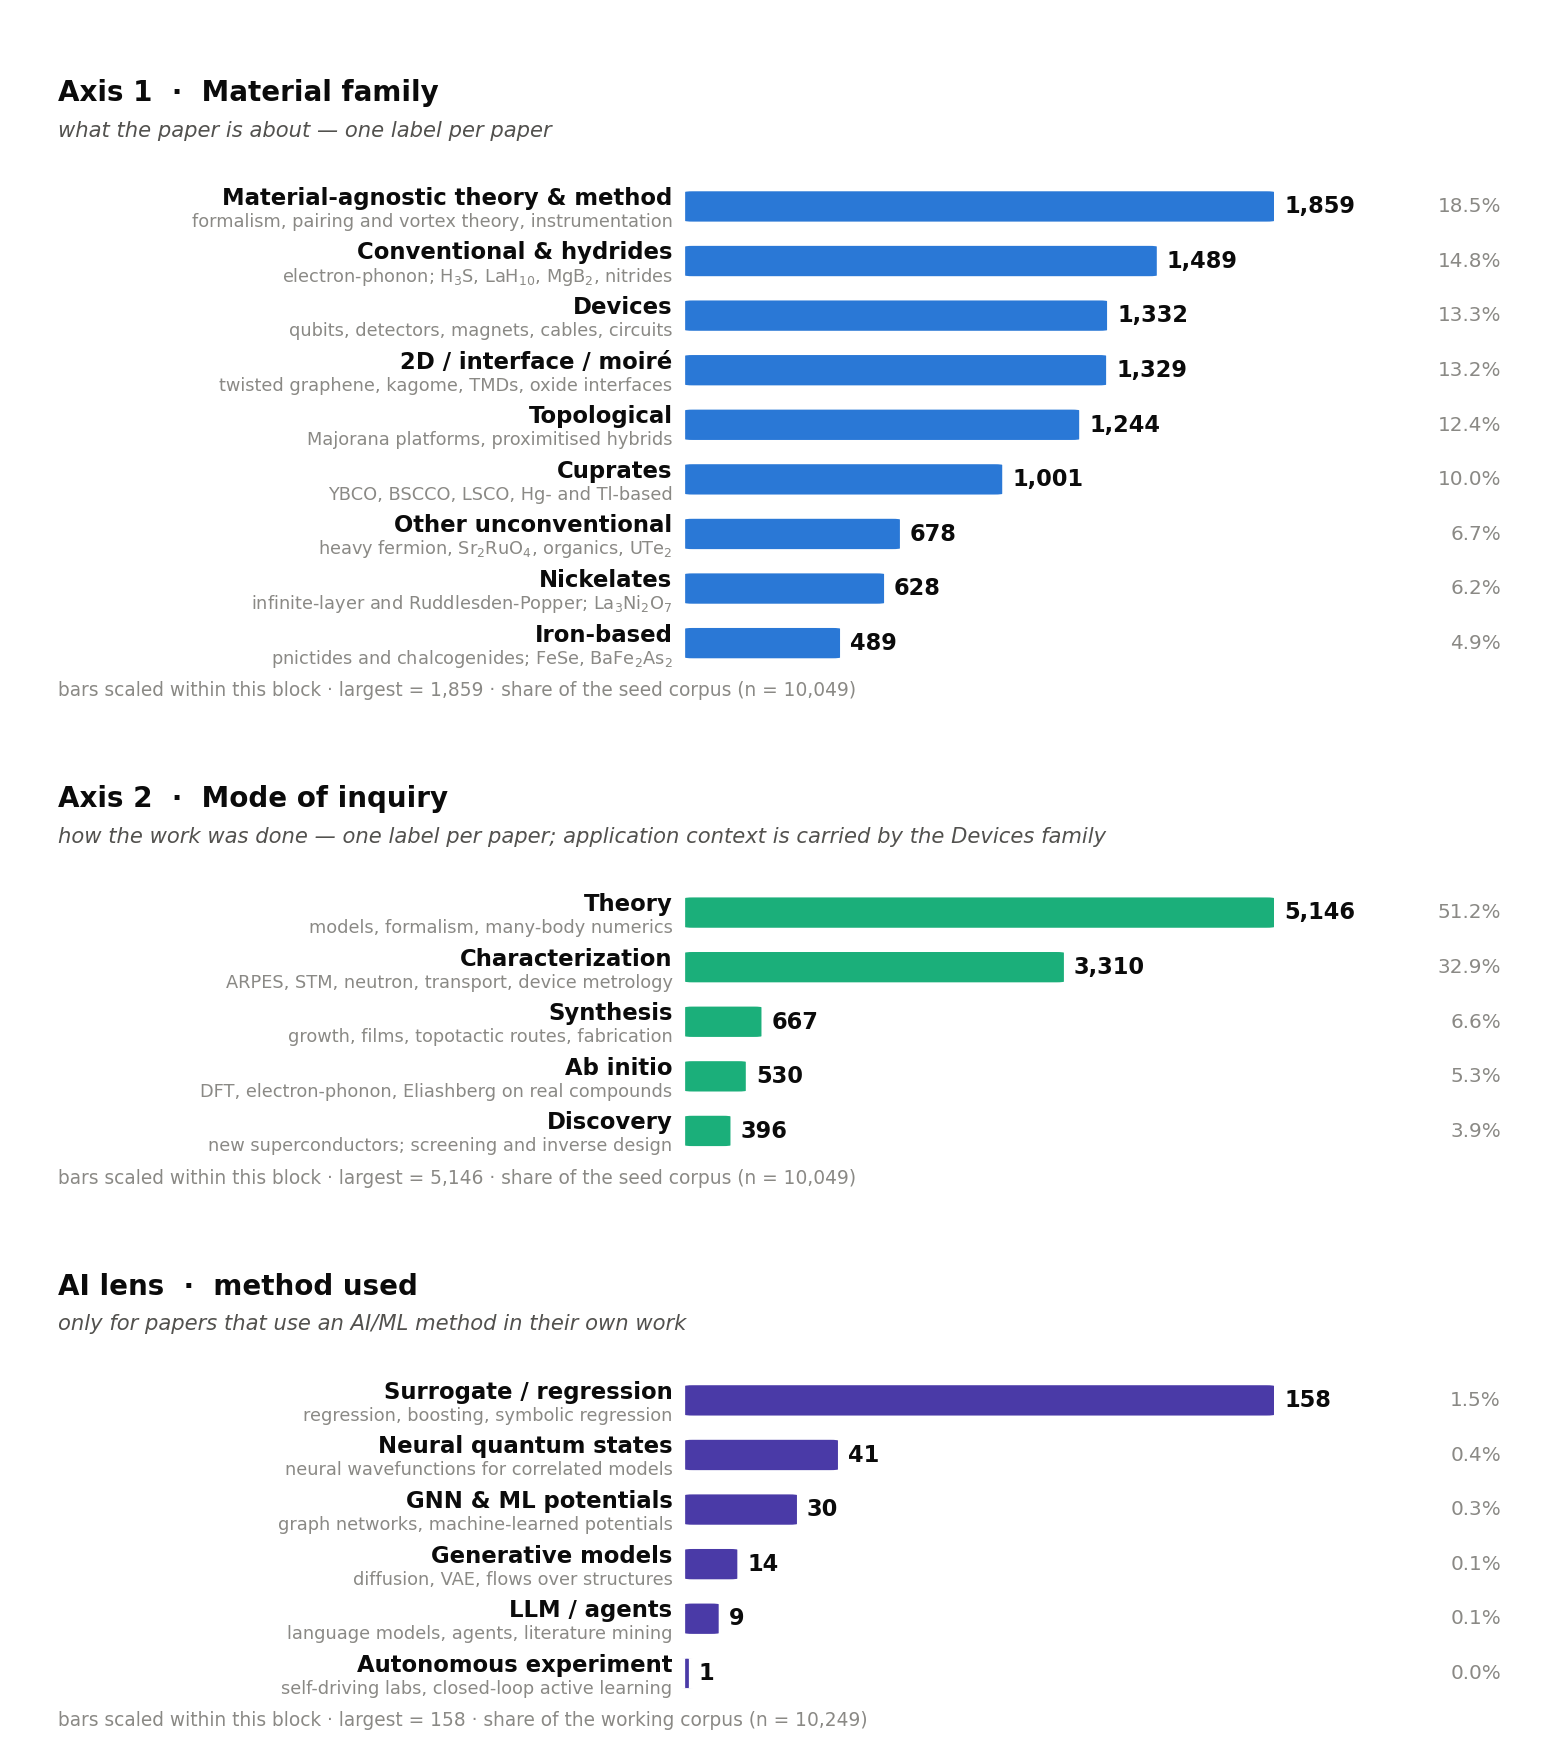
\includegraphics[keepaspectratio,alt={Figure 1: The taxonomy. Every corpus record carries one label from Axis 1 and one from Axis 2; the AI lens applies only to records that use a machine-learning method in their own work.}]{figures/fig1_taxonomy.png}}
\caption*{Figure 1: The taxonomy. Every corpus record carries one label
from Axis 1 and one from Axis 2; the AI lens applies only to records
that use a machine-learning method in their own work.}
\end{figure}

\section{Positioning relative to existing
surveys}\label{positioning-relative-to-existing-surveys}

Two bodies of review literature already cover parts of this ground, and
neither covers the join.

The first is per-family physics reviews. Recent examples treat nickelate
superconductivity \citep{wang2025recent, zhang2026superconductivity} and
the hydride programme. These are authoritative on mechanism and
materials, and they say little about method infrastructure: what data
exists, what is measurable at scale, where a model could be trained or
tested.

The second is machine-learning-for-superconductors reviews. Recent
examples survey materials-informatics approaches to superconductor
discovery \citep{tran2025superconductor}, machine-learning searches for
new superconductors \citep{adiga2025accelerating}, AI-driven
high-throughput screening \citep{gashmard2025ai}, and language-model
workflows for extraction and property prediction
\citep{itani2025large, li2026agentic}. These are organised by method,
and their material scope is dominated by the one task where tabulated
data happens to exist -- predicting \(T_c\) from composition.

This survey takes the join as its subject. It maps the whole field onto
a family-by-mode grid, populates that grid from a systematically
harvested corpus, and then asks of each cell what would have to be true
for a machine-learning method to contribute there. The result is a
statement about where the opportunities are \emph{not}, which the
method-organised reviews cannot make because they only look where the
methods already are.

\section{Corpus construction}\label{corpus-construction}

\textbf{Seed harvest.} Every arXiv preprint listed under
\texttt{cond-mat.supr-con}, as primary category or cross-list, submitted
between 2021-09-01 and 2026-09-07, retrieved month by month through the
arXiv API. This is a systematic, not a keyword, harvest: the selection
criterion is the category label the authors themselves chose. It yields
10,303 records, of which 6,986 carry \texttt{cond-mat.supr-con} as
primary category and 3,317 are cross-listed from elsewhere. Raw
responses are cached per month so the harvest is reproducible.

\textbf{Targeted supplement.} The seed necessarily misses
AI-for-materials work that never touches the superconductivity category.
Two supplementary threads were harvested by keyword: AI applied to
superconductivity from adjacent categories, and general AI-for-materials
infrastructure needed for Section 6. These add 691 records tagged
\texttt{supplement\_t1} and \texttt{supplement\_t2}. \textbf{The
supplement is recency-biased by construction} -- its queries are capped
and sorted by submission date -- so it is excluded from every growth
statistic and from Table 1's family-by-mode counts, where it appears
only as a separate column.

\textbf{Off-topic filtering.} 745 records were flagged as not about
superconductivity and excluded from all statistics. Within the
systematically harvested seed the rate is 254 of 10,303, or
\textbf{2.5\%}, which is this corpus's measured query-bleed. The rate is
far higher in the supplement, as intended: the general AI-for-materials
thread was designed to reach outside the field. After exclusion the
working corpus is \textbf{10,249 records: 10,049 seed and 200
supplement.}

\textbf{Labelling.} Both axes and the AI lens were assigned by a
language-model pass over title and abstract
(\texttt{gemini-3.5-flash-lite}), after keyword rules were measured and
found inadequate. Agreement with a hand-labelled 150-record stratified
sample:

{\def\LTcaptype{none} % do not increment counter
\begin{longtable}[]{@{}lll@{}}
\toprule\noalign{}
labels & family & mode of inquiry \\
\midrule\noalign{}
\endhead
\bottomrule\noalign{}
\endlastfoot
keyword rules & 80.1\% & 70.5\% \\
language-model pass & 85.6\% & 88.4\% \\
\end{longtable}
}

Per-class recall for the model is 96\% (theory), 92\%
(characterization), 92\% (ab initio), 64\% (synthesis) and 54\%
(discovery). The two small classes are the weak ones, and no claim in
this survey rests on their counts alone. The AI lens was validated
separately against 120 hand-labelled records, half drawn from each side
of the rule-based tag: 88\% precision and 81\% recall on the
AI-versus-not decision, 84\% exact agreement on which method.

\textbf{Taxonomy revision, disclosed.} The two agreement figures above
are not measured against the same label set. The task axis originally
carried a sixth value, \texttt{application}; the first labelling round
showed that characterization-versus- application was the dominant
disagreement for the keyword rules and for both benchmarked language
models alike, which identified the value as conflating mode of work with
purpose rather than as a classifier failure. The value was removed, the
146 scored hand labels were remapped accordingly, and the models were
re-scored against the revised set. The 70.5\% rule figure predates that
revision and is reported for completeness rather than as a like-for-like
comparison. The prompt was also sharpened once, after per-class recall
showed synthesis at 55\%, by adding explicit
synthesis-versus-characterization and discovery-versus-ab-initio
boundary rules; the corpus was then relabelled from scratch with the
final prompt.

\textbf{Annotator disclosure.} All hand labels were produced by a single
annotator, in the same working session that built the pipeline. The
figures above are therefore agreement between one human pass and one
model pass, not accuracy against an external ground truth. Corpus,
labels, prompts and scripts are released so that both passes can be
re-run and re-scored.

\textbf{Citation counts.} Citation data comes from OpenAlex, resolved
for 8,280 of the records. Over a five-year window raw counts favour
older work mechanically, so where this survey ranks papers it ranks by
citations per month since submission, and citation counts for work less
than a year old are not read as impact at all.

Table 1: Corpus by material family and mode of inquiry. Counts are seed
records after off-topic filtering; the supplement is listed separately
because it is recency-biased by construction and is excluded from all
trend statistics.

{\def\LTcaptype{none} % do not increment counter
\begin{longtable}[]{@{}
  >{\raggedright\arraybackslash}p{(\linewidth - 14\tabcolsep) * \real{0.1250}}
  >{\raggedleft\arraybackslash}p{(\linewidth - 14\tabcolsep) * \real{0.1250}}
  >{\raggedleft\arraybackslash}p{(\linewidth - 14\tabcolsep) * \real{0.1250}}
  >{\raggedleft\arraybackslash}p{(\linewidth - 14\tabcolsep) * \real{0.1250}}
  >{\raggedleft\arraybackslash}p{(\linewidth - 14\tabcolsep) * \real{0.1250}}
  >{\raggedleft\arraybackslash}p{(\linewidth - 14\tabcolsep) * \real{0.1250}}
  >{\raggedleft\arraybackslash}p{(\linewidth - 14\tabcolsep) * \real{0.1250}}
  >{\raggedleft\arraybackslash}p{(\linewidth - 14\tabcolsep) * \real{0.1250}}@{}}
\toprule\noalign{}
\begin{minipage}[b]{\linewidth}\raggedright
Family
\end{minipage} & \begin{minipage}[b]{\linewidth}\raggedleft
Theory
\end{minipage} & \begin{minipage}[b]{\linewidth}\raggedleft
Ab init.
\end{minipage} & \begin{minipage}[b]{\linewidth}\raggedleft
Discov.
\end{minipage} & \begin{minipage}[b]{\linewidth}\raggedleft
Synth.
\end{minipage} & \begin{minipage}[b]{\linewidth}\raggedleft
Charac.
\end{minipage} & \begin{minipage}[b]{\linewidth}\raggedleft
Seed
\end{minipage} & \begin{minipage}[b]{\linewidth}\raggedleft
Suppl.
\end{minipage} \\
\midrule\noalign{}
\endhead
\bottomrule\noalign{}
\endlastfoot
Conventional & 199 & 237 & 271 & 193 & 589 & \textbf{1489} & 15 \\
Cuprate & 445 & 54 & 7 & 58 & 437 & \textbf{1001} & 2 \\
Iron-based & 95 & 15 & 4 & 58 & 317 & \textbf{489} & 0 \\
Nickelate & 212 & 113 & 20 & 74 & 209 & \textbf{628} & 1 \\
Other unconv. & 320 & 10 & 20 & 22 & 306 & \textbf{678} & 0 \\
2D / moiré & 594 & 74 & 38 & 65 & 558 & \textbf{1329} & 10 \\
Topological & 909 & 14 & 8 & 37 & 276 & \textbf{1244} & 9 \\
Devices & 611 & 4 & 2 & 156 & 559 & \textbf{1332} & 109 \\
Material-agnostic & 1761 & 9 & 26 & 4 & 59 & \textbf{1859} & 54 \\
\textbf{Total} & \textbf{5146} & \textbf{530} & \textbf{396} &
\textbf{667} & \textbf{3310} & \textbf{10049} & \textbf{200} \\
\end{longtable}
}

\begin{figure}
\centering
\pandocbounded{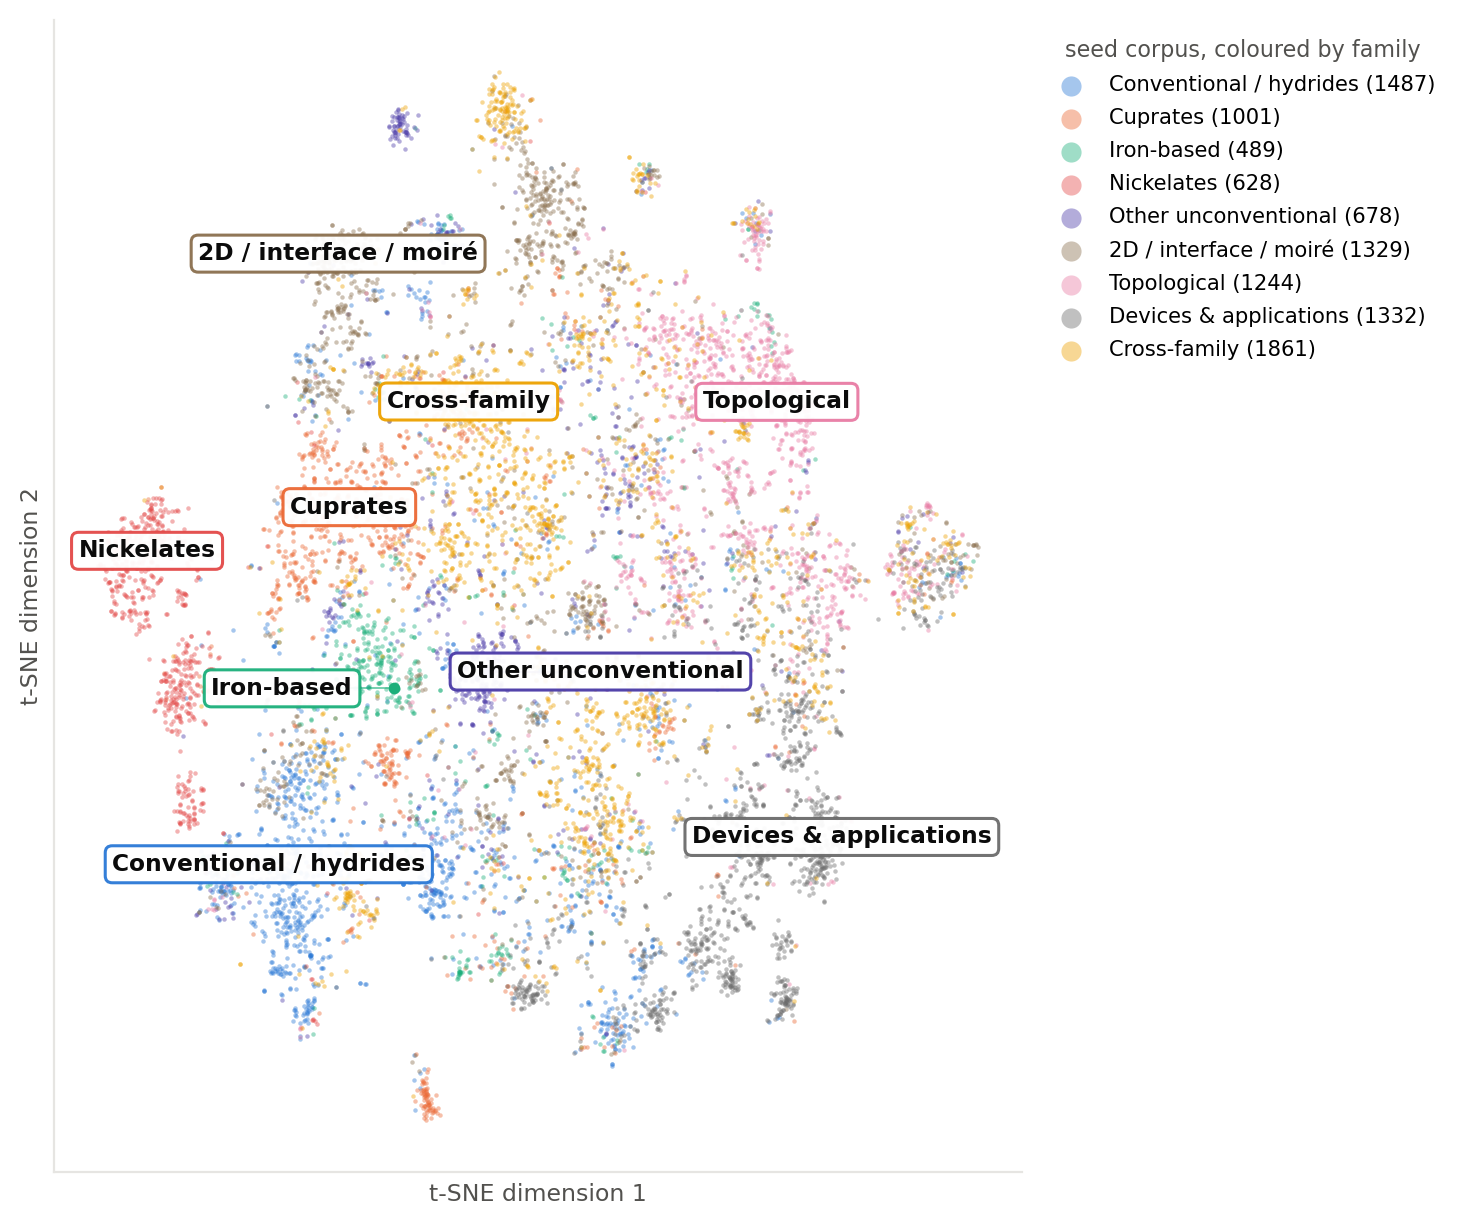
\includegraphics[keepaspectratio,alt={Figure 2: Semantic map of the seed corpus (TF-IDF, truncated SVD, t-SNE), coloured by material family. Per-family counts match Table 1.}]{figures/fig2_semantic_map.png}}
\caption*{Figure 2: Semantic map of the seed corpus (TF-IDF, truncated
SVD, t-SNE), coloured by material family. Per-family counts match Table
1.}
\end{figure}

\textbf{Limitations.} The corpus is arXiv-only, so it inherits arXiv's
coverage: strong in theory and condensed-matter experiment, weaker in
applied-superconductivity engineering that publishes in IEEE venues, and
blind to unpublished industrial work, which matters most for the device
family. Category self-assignment means a paper whose authors did not
cross-list to \texttt{cond-mat.supr-con} is absent from the seed
regardless of content. Labels are single-label where reality is often
multi-label: a paper that grows a crystal and measures it gets one mode,
chosen by which the abstract presents as the contribution.

\section{Material families}\label{material-families}

This section walks Axis 1. Each family is treated for what it is
currently doing, what is open, and -- because that is this survey's
purpose -- what kind of data it generates. Counts are seed-corpus counts
from Table 1 and Figure 2.

\begin{figure}
\centering
\pandocbounded{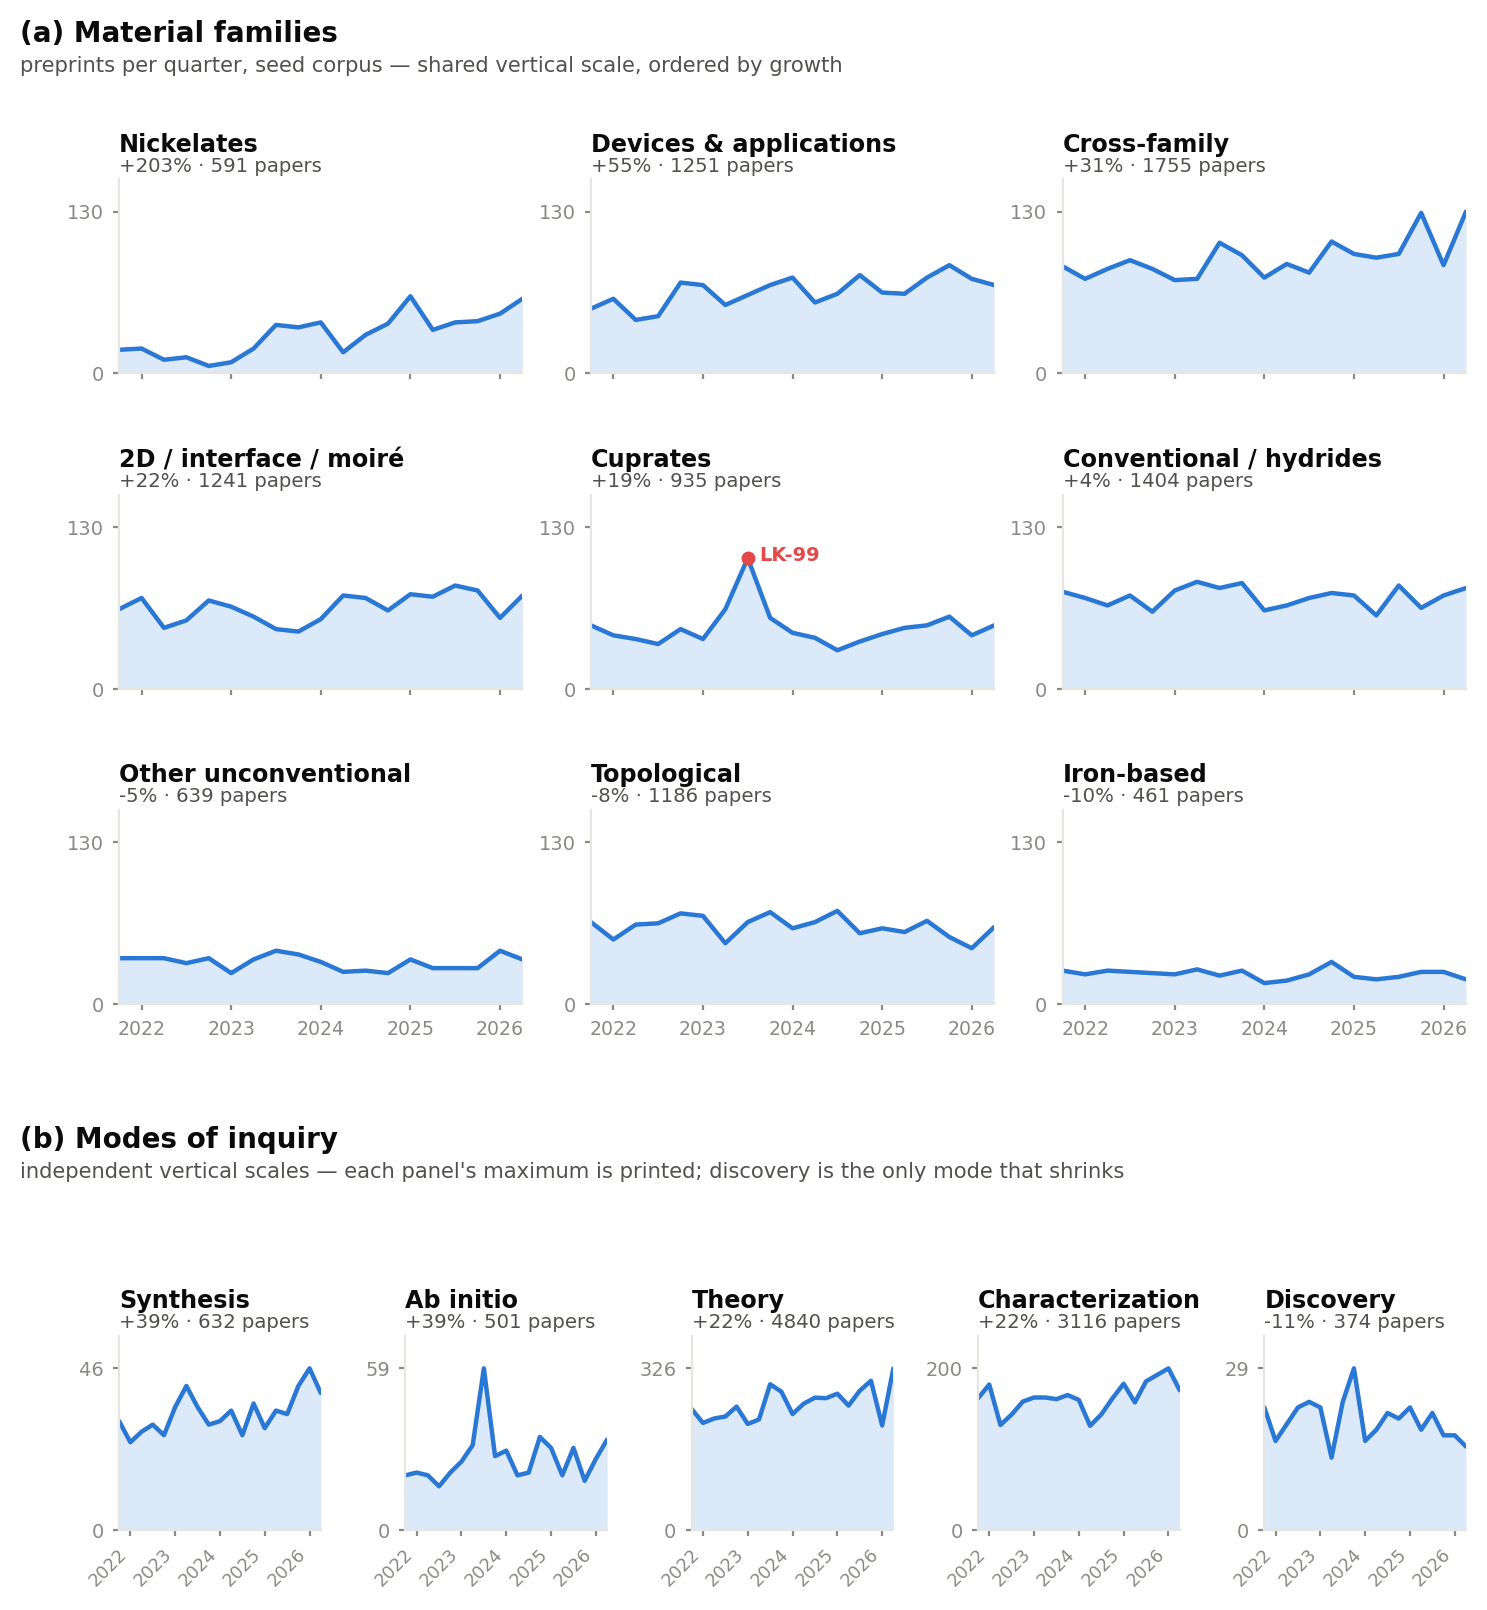
\includegraphics[keepaspectratio,alt={Figure 3: Quarterly submissions by material family (a) and mode of inquiry (b), seed records only. Both partial endpoint quarters are omitted. The cuprate spike in 2023Q3 is the LK-99 replication burst discussed in Section 3.}]{figures/fig3_growth_timeline.png}}
\caption*{Figure 3: Quarterly submissions by material family (a) and mode
of inquiry (b), seed records only. Both partial endpoint quarters are
omitted. The cuprate spike in 2023Q3 is the LK-99 replication burst
discussed in Section 3.}
\end{figure}

\section{Nickelates: the fast-moving
family}\label{nickelates-the-fast-moving-family}

Nickelates are the smallest of the named families in this corpus (628
seed records) and the fastest-growing (Figure 3a). The line begins
outside the window with superconductivity in an infinite-layer nickelate
thin film \citep{li2019superconductivity}, and turns sharply with the
report of superconductivity near 80 K in La\(_3\)Ni\(_2\)O\(_7\) above
14 GPa \citep{sun2023superconductivity}.

What followed is a useful case study in how a modern materials claim is
stabilised. The original report lacked zero resistance; that was
supplied under a liquid pressure medium, together with strange-metal
\(T\)-linear resistivity whose coefficient tracks the superconducting
transition under pressure \citep{zhang2023high}. Polycrystalline samples
then reproduced the effect, reaching zero resistivity at 9 GPa and 35.6
K at 14.5 GPa \citep{wang2023pressurea}. In parallel, careful
high-pressure work reported that the superconductivity is filamentary
rather than bulk, and tied the inconsistent reproducibility to oxygen
content \citep{zhou2023investigations}. Bulk superconductivity with zero
resistivity and a Meissner signal was subsequently reported in
flux-grown La\(_2\)SmNi\(_2\)O\(_{7-\delta}\) single crystals, at 92 K
onset and 73 K zero-resistance at 21.6 GPa \citep{li2025bulk}.

The pressure requirement is the family's practical obstacle, and
thin-film strain engineering is the route around it. Compressively
strained (La,Pr)\(_3\)Ni\(_2\)O\(_7\) films on SrLaAlO\(_4\) gave an
ambient-pressure onset of 45 K with a
Berezinskii-Kosterlitz-Thouless-like transition at 9 K
\citep{zhou2024ambient}, and a subsequent extreme non-equilibrium growth
regime raised the onset to about 63 K with zero resistance near 37 K
\citep{zhou2025superconductivity}. The gap between onset and
zero-resistance temperatures in these films is exactly the definitional
issue flagged in Section 2, and it is the reason both numbers are quoted
here.

Theory moved at the same pace, converging quickly on bilayer two-orbital
models built from first-principles band structures, with \(s_\pm\)
pairing driven by the Ni \(d_{z^2}\) orbital and its interlayer exchange
\citep{gu2023effective, luo2023bilayer, sakakibara2023possible, shen2023effective}.
\textbf{For AI purposes the nickelate story is instructive in a
discouraging way}: the rate-limiting steps were sample quality, oxygen
stoichiometry and pressure technique. None of them is a prediction
problem.

\section{Conventional superconductors and hydrides: prediction that
outruns
measurement}\label{conventional-superconductors-and-hydrides-prediction-that-outruns-measurement}

The conventional family is the corpus's largest single-material grouping
(1,489 seed records) and the only one where computational prediction
routinely precedes experiment. Its anchors are the 203 K report in the
sulfur hydride system \citep{drozdov2015conventional} and the lanthanum
superhydride results near 250-260 K
\citep{drozdov2019superconductivity, somayazulu2019evidence}. Within the
window the programme continues at megabar pressures, with reports in
cerium superhydrides \citep{semenok2023evidence, cao2024probing}, Ca-Mg
ternary superhydrides above 180 K \citep{cai2023superconductivity}, and
a claim of superconductivity with onset between 271 and 298 K in a
La-Sc-H system at 195-266 GPa \citep{song2025room}. That last claim is
recent, singular and not independently replicated at the time of
writing, and the retraction record discussed below is the reason to say
so explicitly rather than to quote the number alone.

This family also carries the field's heaviest evidential burden. Two
prominent claims were retracted
\citep{snider2020retracted, dasenbrock2023retracted}. The Lu-N-H episode
is still unsettled rather than closed: one group reported resistance
measurements in good agreement with the original transition temperature
and its pressure dependence \citep{salke2023evidence}, while several
others reported no superconductivity in samples they prepared, and
first-principles modelling of the plausible parent structures concluded
that the observed Raman spectrum matches LuH\(_3\), that the
pressure-driven colour change is an optical property of LuH\(_2\)
requiring no structural transition, and that neither compound
superconducts at high temperature \citep{dangic2023ab}. Methodological
argument continues over what counts as proof at these pressures,
including whether flux-trapping magnetisation demonstrates
superconductivity in H\(_3\)S \citep{tallon2024flux}.

This family is where AI-assisted screening is concentrated, for a reason
Section 6 formalises: the target quantity is the Eliashberg \(T_c\),
which is computable, so a model can be trained and checked without a
diamond anvil cell. The distribution in Table 1 shows the consequence --
conventional systems carry 237 of the corpus's 530 ab initio records and
271 of its 396 discovery records, more than any other family in both.

\section{Cuprates: mature physics, and a cautionary
spike}\label{cuprates-mature-physics-and-a-cautionary-spike}

Cuprates account for 1,001 seed records, dominated by characterization
(437) and theory (445), with only 7 discovery records. Forty years after
the original observation \citep{bednorz1986possible}, the open question
is still the mechanism, and the work is correspondingly weighted toward
precision measurement of known compounds and model studies of the doped
Hubbard and \(t\)-\(J\) systems.

The family's most striking corpus feature is an artefact worth
reporting. Ranked by citations per month, the top of the cuprate list is
not cuprate physics at all: it is LK-99, the Cu-substituted lead apatite
claimed as a room-temperature ambient-pressure superconductor
\citep{lee2023lk99, lee2023superconductor}. The classifier placed these
in the cuprate family because the material is a copper oxide compound,
which is defensible chemically and wrong physically. The episode is
visible in Figure 3a as a sharp cuprate spike in 2023Q3, and it resolved
quickly: phase-pure single crystals proved highly insulating and
optically transparent with no transition anomalies, ruling out
superconductivity \citep{puphal2023single}. The episode is also a good
example of how first-principles work enters a live controversy on both
sides: Griffin's density-functional calculations identified correlated
isolated flat bands at the Fermi level, noting these as a signature
associated with high transition temperatures \citep{griffin2023origin},
which made the compound worth taking seriously even as the crystals were
failing to superconduct. The replication burst is the most compressed
example in this corpus of the field's self-correction working, and of
how quickly a high-visibility claim distorts the literature's shape.

\section{Iron-based superconductors:
consolidation}\label{iron-based-superconductors-consolidation}

At 489 seed records, iron-based systems are the smallest named family
and the most stable in Figure 3a. Fifteen years after the founding
report \citep{kamihara2008iron}, the work is consolidation:
orbital-selective pairing assisted by Hund's coupling in
Ba\(_{1-x}\)K\(_x\)Fe\(_2\)As\(_2\) \citep{corbae2025hunds},
sign-reversal gap structure in FeTe\(_{0.55}\)Se\(_{0.45}\)
\citep{hou2025distinct}, time-reversal-symmetry-breaking states
\citep{bartl2025evidence}, and vortex-matter studies
\citep{sanchez2023disordered, iguchi2023observation}. The family is
characterization-dominated (317 of 489), and it is the one where the
phase diagram is best mapped, which makes it the most plausible
near-term source of the labelled spectral datasets Section 6 argues for.

\section{Two-dimensional, interface and moiré
systems}\label{two-dimensional-interface-and-moiruxe9-systems}

This family (1,329 seed records) is the corpus's second-largest and its
most methodologically distinctive: superconductivity here is tuned
electrostatically rather than chemically. It splits into two active
lines. The moiré line descends from magic-angle twisted bilayer graphene
\citep{cao2018unconventional} and now covers Bernal bilayer graphene
with strong spin-orbit coupling \citep{holleis2023nematicity}, twisted
trilayers, and rhombohedral multilayers, with heavy-fermion-style
modelling of the correlated regime \citep{lau2023topological}. The
kagome line runs through AV\(_3\)Sb\(_5\) \citep{jiang2021kagome}, where
charge order and its competition with superconductivity dominate
\citep{kang2022charge, hu2022coexistence}, and unusual flux quantization
in units of \(h/4e\) and \(h/6e\) has been reported in ring devices
\citep{ge2022charge}. Whether the charge-ordered state breaks
time-reversal symmetry remains disputed: high-resolution Sagnac Kerr
measurements on CsV\(_3\)Sb\(_5\) found no signal to a 30 nanoradian
noise floor, leading those authors to conclude that
time-reversal-symmetry breaking in the charge-ordered state is highly
unlikely \citep{saykin2022high}. Titanium-based analogues extend the
family \citep{yang2022superconductivitya}.

For this survey the important property is that these systems are
device-like: each sample is a fabricated stack, gate-tunable, and
measured with electrical transport. That generates dense, structured,
parameterised data of exactly the kind a model can use -- and
simultaneously makes each sample expensive and non-identical, which is
why the family scores well on data and poorly on validation cost in
Figure 5.

\section{Topological
superconductivity}\label{topological-superconductivity}

At 1,244 seed records, this family is theory-heavy (909 of 1,244) in a
way no other family matches. The experimental programme has consolidated
around quantum-dot-based minimal Kitaev chains
\citep{dvir2022realization, tsintzis2023roadmap, bordin2023crossed}
rather than the earlier bare-nanowire route, which is itself a response
to a decade of contested zero-bias-peak evidence. Josephson diode
physics runs through this family and into devices
\citep{mazur2022gate, lotfizadeh2023superconducting}.

The theory-to-experiment ratio here is the sharpest warning in the
corpus about reading activity as progress. It is also, from the AI
standpoint, the least tractable cell: what a model would predict is
unclear when the disagreement is about what a measurement means.

\section{Other unconventional
systems}\label{other-unconventional-systems}

This family (678 seed records) collects heavy-fermion, ruthenate,
organic and noncentrosymmetric compounds. Two currents dominate the
window: UTe\(_2\), where triplet superconductivity is studied in
progressively cleaner crystals \citep{wu2023enhanced} following the
original spin-triplet report \citep{ran2019nearly}, and where an earlier
claim of time-reversal-symmetry breaking did not survive: Kerr
measurements across samples grown by two different routes found no
evidence for a spontaneous signal \citep{ajeesh2023fate}, and the
arrival of altermagnetism as a cross-cutting concept
\citep{mazin2022notes}, now reaching into diode effects
\citep{schrade2026altermagnetic} and Cr-based kagome systems
\citep{xu2023altermagnetic, peng2024flat}. This family is the clearest
case of small-sample physics: crystal quality is the experiment, which
is why it is characterization-heavy (306) and nearly synthesis-free in
the corpus (22).

\section{Devices and applications}\label{devices-and-applications}

At 1,332 seed records this family is large, and it is the one whose
corpus representation is least trustworthy: much applied
superconductivity publishes in IEEE venues that arXiv's
\texttt{cond-mat.supr-con} category does not capture, and industrial
qubit work is under-posted. What the corpus does capture is
materials-limited qubit physics -- dielectric loss in nitride films
\citep{deng2022titanium}, niobium film structure and circuit losses
\citep{drimmer2024effect}, quasiparticle poisoning from phonon bursts
\citep{anthonypetersen2022stress} -- along with scaling roadmaps
\citep{mohseni2024build, aasen2025roadmap}.

This is where the survey's AI story is most positive, and Section 5
explains why: the family's measurements are machine-generated,
standardised and high-volume, so characterization models have a real
training signal. It is the only cell in Figure 5 that scores 3 on data
availability for a measurement task.

\section{Material-agnostic theory and
method}\label{material-agnostic-theory-and-method}

The largest single label in the corpus is not a material at all: 1,859
seed records are material-agnostic theory, formalism and
instrumentation. That a residual category is modal is a finding rather
than a bookkeeping artefact, and the sample inspection behind Table 1
shows what it contains -- Josephson and diode phenomenology
\citep{nadeem2023superconducting, kochan2023phenomenological, wang2022symmetry},
Hubbard-model studies not tied to one compound
\citep{xu2023coexistence}, topological field theory of the
superconducting state \citep{verresen2022higgs, thorngren2023higgs},
quantum-geometric contributions to coupling \citep{yu2023nontrivial},
and measurement methodology.

The AI relevance is direct: this is where neural quantum states live
(Section 5), and it is the only large cell whose validation is internal
to a calculation.

\section{Assessment}\label{assessment}

Across families, two patterns matter for what follows. First, the
families differ less in how much data they produce than in whether that
data has a machine-readable target: hydrides have a computable \(T_c\),
devices have instrument telemetry, and cuprates have four decades of
spectra with no agreed quantity to predict. Second, the step that gates
progress is overwhelmingly experimental -- sample quality in nickelates
and UTe\(_2\), pressure technique in hydrides, stack fabrication in
moiré systems, and film chemistry in qubits. Section 4 turns from what
is studied to how, and asks what infrastructure each mode of inquiry
actually has.

\section{Modes of inquiry and their data
infrastructure}\label{modes-of-inquiry-and-their-data-infrastructure}

Axis 1 says what the field studies. Axis 2 says how, and it is the axis
that determines whether a machine-learning method has anything to attach
to. This section takes each mode in turn and asks the same question:
what does this mode produce that a model could learn from or be tested
against?

\section{Theory: 5,146 records, no target
quantity}\label{theory-5146-records-no-target-quantity}

Theory is the corpus's largest mode -- half the seed. It spans model
Hamiltonians, pairing symmetry analysis, Ginzburg-Landau and
Bogoliubov-de Gennes treatments, quantum Monte Carlo, DMRG and dynamical
mean-field theory. The output of a theory paper is an argument, a phase
diagram or a mechanism, and none of those is a label.

The exception is where theory is a \emph{computation} rather than an
argument: solving a model whose Hamiltonian is written down but whose
ground state is not known. There a model can be trained and scored,
which is why neural quantum states occupy this mode (Section 5) and
nothing else in the AI literature does. The distinction matters for
Section 6: theory is not one cell for AI purposes but two, and only the
computational half is addressable today.

\section{Ab initio: 530 records, the field's one mature
pipeline}\label{ab-initio-530-records-the-fields-one-mature-pipeline}

Ab initio work is the smallest mode after discovery, and it is the only
one with an end-to-end, standardised, machine-consumable pipeline: DFT
for the electronic structure, density-functional perturbation theory for
phonons, Migdal-Eliashberg or superconducting density-functional theory
for \(T_c\), with anharmonicity treated through the stochastic
self-consistent harmonic approximation where it matters. The inputs are
structures, the outputs are numbers, both are reproducible, and the
convergence parameters are arguable but conventional.

This is why the AI-screening literature lives here. A dataset of about
7,000 electron-phonon calculations was sufficient to train a model that
then screened 200,000 compounds \citep{cerqueira2023sampling}; the same
infrastructure supported the million-compound search behind the
Mg\(_2\)XH\(_6\) proposal \citep{sanna2023prediction} and the
36-million-structure hydride exploration \citep{wang2025discoverya}.
\textbf{No other mode in this survey has a comparable substrate.} The
cost is the well-known one: the pipeline is trustworthy for
phonon-mediated pairing and does not transfer to the correlated
families, which is exactly why 237 of the 530 ab initio records sit in
the conventional family and only 54 in cuprates.

\section{Discovery: 396 records, and an ambiguity that
matters}\label{discovery-396-records-and-an-ambiguity-that-matters}

Discovery is the smallest mode, and it is internally split in a way the
count hides. Some of these papers report a new superconductor that was
made and measured; others report a computational screen whose candidates
remain unsynthesised. Section 2 fixed the vocabulary for this
distinction, and Section 5 shows why it is load-bearing: the screening
literature's headline numbers are all of the second kind.

The data infrastructure for this mode is the weakest part of the field's
machine-learning story, and it is worth being concrete. The workhorse
resource is the SuperCon database of composition-\(T_c\) pairs, which
carries no crystal structures. The 3DSC dataset was built specifically
to fix that, augmenting superconductors with approximate
three-dimensional structures and, importantly, including tested
non-superconductors \citep{sommer20223dsc}. General-purpose materials
infrastructure -- JARVIS, with more than 80,000 materials, unified force
fields and graph-network design tools \citep{wines2023recent}; the
Materials Project; GNoME's stable-structure set
\citep{merchant2023scaling} -- supplies structures and formation
energies but not superconducting labels. The recent language-model
extraction of 78,203 experimental records \citep{itani2025large} is the
largest attempt to close that gap from the literature side.

Two structural problems remain, and neither is a modelling problem.
Negative results are scarce, in two distinct senses that are easy to
conflate. Computed non-superconductors can be generated in bulk, and the
one large compilation in this corpus -- 53,196 entries -- was assembled
as a deliberate remedy for classifier training \citep{gashmard2025ai};
the 3DSC dataset likewise includes tested non-superconductors
\citep{sommer20223dsc}. Experimentally \emph{attempted and failed}
syntheses are a different and almost entirely missing record, and it is
that second kind the synthesis mode needs. And the labels are contested
at the top of the range, where retractions
\citep{snider2020retracted, dasenbrock2023retracted} and unreplicated
claims \citep{lee2023lk99} sit precisely in the high-\(T_c\) region a
model is being asked to extrapolate into.

\section{Synthesis: 667 records, and almost no machine-readable
trace}\label{synthesis-667-records-and-almost-no-machine-readable-trace}

Synthesis is where superconductivity is actually rate-limited, as
Section 3 found in family after family. It is also the mode with the
least usable data infrastructure in the entire survey. A synthesis paper
reports a recipe in prose -- precursors, temperatures, atmospheres,
durations, substrate, annealing schedule -- and reports it only for the
attempts that worked. Failed attempts are not published, so the negative
half of the training set does not exist.

The mode is also technique-diverse in a way that resists automation. The
corpus's synthesis records include topotactic reduction of nickelate
films, diamond-anvil-cell synthesis at hundreds of gigapascals,
molecular-beam epitaxy, flux growth, and mechanical stacking of
exfoliated flakes. The autonomous-laboratory programme
\citep{szymanski2023autonomous} targets none of these; it targets bulk
oxide powder synthesis, and even there its claims have been disputed
\citep{leeman2024challenges}.

The corpus's own signature is stark: \textbf{one AI-tagged synthesis
paper.} Section 6 argues that the tractable target here is not
automating synthesis but predicting synthesizability.

\section{Characterization: 3,310 records, abundant data in unusable
form}\label{characterization-3310-records-abundant-data-in-unusable-form}

Characterization is the second-largest mode and the field's main
empirical output: ARPES, scanning tunnelling spectroscopy, neutron
scattering, muon spin rotation, NMR, optical and terahertz spectroscopy,
transport, specific heat, and magnetometry.

The data situation here is the survey's central irony. This mode
produces enormous quantities of exactly the structured, high-dimensional
data that machine learning handles well, and almost none of it is
available in a form a model can consume. Raw spectra are rendered as
figures in PDFs, per-group formats are undocumented, and supplementary
files lack schemas. We did not survey data-availability practice
directly, so we state the weaker claim this corpus supports: among the
characterization papers read for this survey we encountered no shared
convention for releasing an ARPES cut or an STM map as an array with its
acquisition parameters, and no repository playing the role that
structural databases play for computed materials. Where such data does
exist as a byproduct of machine operation -- qubit readout traces,
detector counts -- machine-learning methods appeared quickly and work
(Section 5).

The tasks are well-posed: inferring a gap structure from a spectrum,
separating overlapping phases in a diffraction pattern, denoising
quasiparticle interference, segmenting features in a microscopy image.
Several are inverse problems with known forward models, which is the
most favourable situation a learning method can be handed. What is
missing is the dataset, not the method.

\section{Assessment}\label{assessment-1}

Ranking the modes by how ready their data is inverts the ranking by how
much attention they get from the machine-learning literature. Ab initio
work has a mature pipeline and a computable target, and it is where the
screening papers concentrate -- correctly. Characterization has abundant
data, well-posed inverse problems and cheap validation, and it is barely
represented. Synthesis has the field's real bottleneck and essentially
no data at all, and it attracts the most ambitious claims. Theory is
half-addressable, and the addressable half is quietly productive.
Section 6 turns these observations into a per-cell assessment.

\section{What AI has actually done in
superconductivity}\label{what-ai-has-actually-done-in-superconductivity}

\section{How rare it still is}\label{how-rare-it-still-is}

The first thing the corpus says about machine learning in
superconductivity is how little of it there is. Of the 10,049 on-topic
preprints in the systematic seed, \textbf{120 use a machine-learning
method in their own work: 1.2\%.} The count grows across the four
complete calendar years in the window -- 13 in 2022, 19 in 2023, 22 in
2024, 38 in 2025 -- but from a base so low that even a tripling leaves
the field's daily practice essentially untouched. A recent review of
computational superconductor discovery reaches the same conclusion from
the opposite direction, describing AI and machine-learning efforts in
this field as remaining ``in its infant stage'' while the predictive
work continues to be carried by Migdal-Eliashberg theory and its
first-principles implementations \citep{tran2025superconductor}.

The distribution across modes of inquiry is more revealing than the
total. Counting the AI-tagged records across the whole working corpus,
seed and supplement together (Figure 4): 124 theory, 64 discovery, 48
characterization, 16 ab initio, and \textbf{1 synthesis.} Machine
learning in this field is something that happens to a calculation or to
a dataset, almost never to a furnace.

\begin{figure}
\centering
\pandocbounded{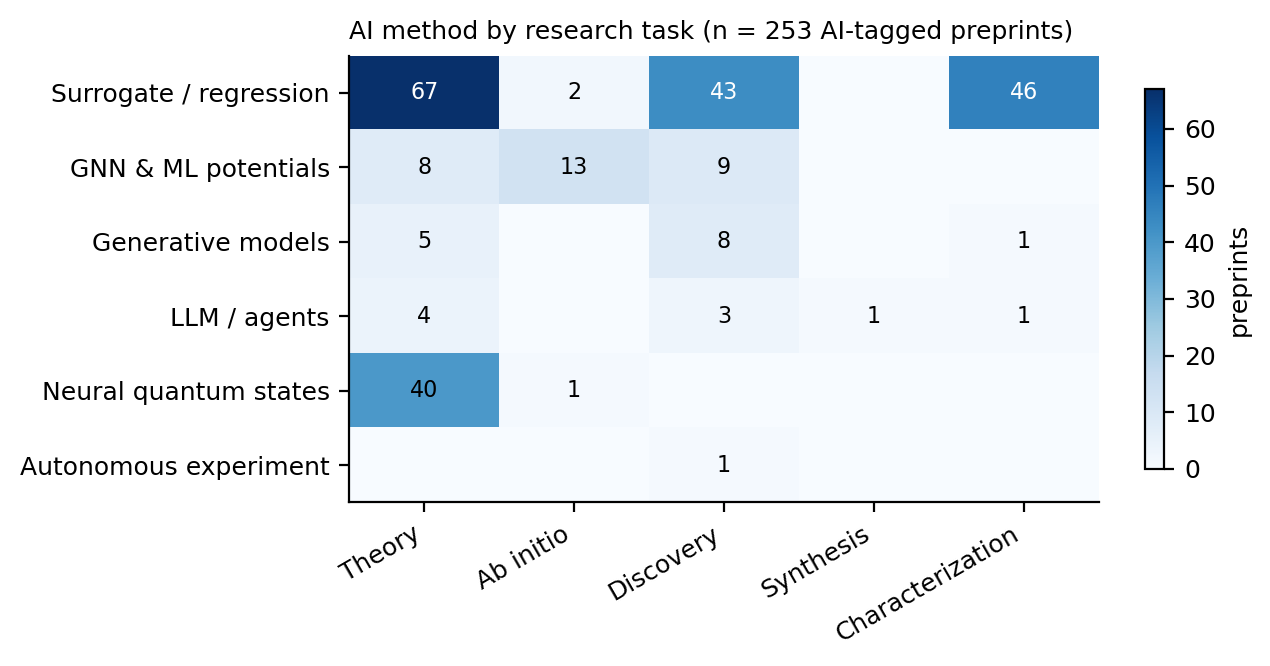
\includegraphics[keepaspectratio,alt={Figure 4: AI-method usage by mode of inquiry across the working corpus. Synthesis carries a single record.}]{figures/fig4_ai_method_task.png}}
\caption*{Figure 4: AI-method usage by mode of inquiry across the working
corpus. Synthesis carries a single record.}
\end{figure}

\section{\texorpdfstring{Predicting \(T_c\), and what the screening
pipelines actually
deliver}{Predicting T\_c, and what the screening pipelines actually deliver}}\label{predicting-t_c-and-what-the-screening-pipelines-actually-deliver}

The oldest and densest thread predicts \(T_c\) from composition or
structure. Its anchors predate this survey's window: a composition-based
classifier and regressor trained on the SuperCon database
\citep{stanev2018machine}, and a widely reused statistical model built
on chemical-formula features \citep{hamidieh2018data}. Both are honest
about scope. The latter predicts a transition temperature only for
materials already known to superconduct, which is a different problem
from finding new ones.

Within the window, the productive form of this thread is not the
regressor alone but the regressor used as a filter in front of
density-functional perturbation theory. The clearest example screens
roughly 200,000 metallic compounds on or near the convex hull with a
model trained on about 7,000 electron-phonon calculations, validates the
survivors with first-principles calculations, and reports 545 compounds
with \(T_c\) above 10 K \citep{cerqueira2023sampling}. The same group
applied the workflow to ambient- pressure hydrides in a set of more than
150,000 compounds, finding around 50 systems above 20 K, and reported
that most of them sit slightly off the convex hull, so synthesis would
need conditions away from ambient equilibrium
\citep{cerqueira2024searching}. A companion study screened over a
million compounds and proposed the thermodynamically stable
Mg\(_2\)XH\(_6\) family, with X = Rh, Ir, Pd or Pt, at 45-80 K and above
100 K with electron doping of the platinum compound
\citep{sanna2023prediction}. A deep-learning framework explored about 36
million ternary hydride structures across 29 elements and identified 144
candidates above 200 K at 200 GPa, 129 of them new
\citep{wang2025discoverya}.

These are substantial results, and they are all predictions in this
survey's sense. None of the four papers reports a synthesised, measured
superconductor. What the machine learning buys is the ratio of
candidates examined to calculations run: the model is a cheap surrogate
that lets an expensive but trusted method be pointed somewhere useful.
That is a real contribution, and it is a narrower one than ``AI
discovers superconductors'' suggests.

\section{Generative and language-model
approaches}\label{generative-and-language-model-approaches}

Generative models entered the field along the path they took in
materials science generally, where diffusion models over atom types,
coordinates and the periodic lattice became the standard instrument for
proposing crystal structures under property constraints
\citep{zeni2025mattergen}. An inverse-design workflow combining
pre-trained models, diffusion and first-principles calculation reported
74 dynamically stable materials with model-predicted \(T_c\) at or above
15 K, singling out B\(_4\)CN\(_3\) at 24.08 K under 5 GPa and
B\(_5\)CN\(_2\) at 15.93 K at ambient pressure
\citep{han2024invdesflow}. The same engine later proposed cubic
Li\(_2\)AuH\(_6\), with a calculated ambient-pressure \(T_c\) near 140 K
and a suggested synthesis route from LiAu and LiH
\citep{ouyang2025high}. Again: calculated, not measured.

Language models arrived more recently and in two distinct roles. The
first is extraction. A language-model workflow built an experimental
database of 78,203 records covering 19,058 unique compositions from the
literature, then fine-tuned open-source models to classify
superconductors, predict \(T_c\), and generate compositions conditioned
on a target \(T_c\) \citep{itani2025large}. The fine-tuned models
performed comparably to feature-based baselines and sometimes better;
28\% of the generated compositions were novel; applying the predictors
to the GNoME database \citep{merchant2023scaling} surfaced unreported
candidates above 10 K. The authors label these candidates unverified,
which is the correct description and a rarer one than it should be.

The second role is orchestration. An agentic framework couples a
billion-parameter atomic model for numerical work to language models for
planning, rediscovers 66 experimentally verified superconductors absent
from the SuperCon3D database, and screens 2.4 million equilibrium
crystals in 28 GPU hours \citep{li2026agentic}. It then does the thing
the rest of this literature does not: \textbf{four proposed compounds
were synthesised and measured} -- Zr\(_3\)ScRe\(_8\) at \(T_c\) = 6.5 K,
HfZrRe\(_4\) at 5.9 K, Zr\(_4\)VRe\(_7\) at 3.5 K, and
Hf\(_{21}\)Re\(_{25}\) at 2.5 K. These transition temperatures are low,
and that is the point worth holding onto. The one clearly closed loop in
the recent literature closed on compounds an order of magnitude below
the temperatures the screening papers advertise.

The earlier closed-loop demonstration is worth reading alongside it.
Four cycles of prediction, experimental test and retraining more than
doubled the success rate of superconductor discovery, found a new
superconductor in the Zr-In-Ni system, and recovered five
superconductors absent from the training data \citep{pogue2022closed}.
Its lesson is about feedback rather than about model class.

\section{Neural quantum states and the theory
side}\label{neural-quantum-states-and-the-theory-side}

The largest AI-tagged mode in the corpus is theory, and within it neural
quantum states are the most self-contained thread. Building on the
demonstration that neural networks can represent many-body wavefunctions
\citep{carleo2017solving}, recent work has pushed the ansatz toward the
models superconductivity actually cares about: the two-dimensional
\(t\)-\(J\) model at finite doping \citep{lange2024simulating}, the
\(t\)-\(t'\) Hubbard model with symmetry-preserving architectures
\citep{rende2026superconductivity}, and the Hofstadter-Hubbard model at
scale \citep{roth2026large}. This thread is unusual in the survey
because its validation is internal: a variational energy can be compared
against other methods without anyone growing a crystal. That is
precisely why it moves faster than the rest.

\section{Characterization: the quiet, working
case}\label{characterization-the-quiet-working-case}

Characterization is where machine learning is least discussed and most
routinely useful. The pattern is a model that turns an instrument's raw
output into a physical quantity: unsupervised learning of nematicity
from scanning-tunnelling data on magic-angle bilayer graphene
\citep{taranto2022unsupervised}, convolutional networks detecting charge
jumps in superconducting qubits in real time
\citep{gaytanvillarreal2026real}, and machine-learned qubit readout
deployed on FPGAs for mid-circuit measurement
\citep{vora2024ml, otting2026multi}. These papers rarely present
themselves as AI-for-science. They are instrument engineering, they are
validated against a ground truth the instrument already provides, and
they work.

\section{The critical literature}\label{the-critical-literature}

Three strands of criticism bear directly on how the results above should
be read, and a survey that omitted them would misrepresent the field.

The first is about what a computational ``discovery'' is worth.
Examining the claims of the GNoME work, Cheetham and Seshadri report
``scant evidence for compounds that fulfill the trifecta of novelty,
credibility, and utility'', and conclude that while the methods hold
promise there is ``a great need to incorporate domain expertise in
materials synthesis and crystallography''
\citep{cheetham2024artificial}. The second concerns autonomous
synthesis. Taking the A-Lab report of 43 autonomously discovered novel
materials \citep{szymanski2023autonomous} as their example, Leeman and
co-workers examined all 43 synthetic products, identified four recurring
shortfalls in the analysis, and concluded that no new materials had been
discovered in that work \citep{leeman2024challenges}. Neither critique
says the programme is worthless. Both say the validation step is where
the difficulty lives, which is the same thing this survey's corpus says
about superconductivity specifically.

The third strand is superconductivity's own reproducibility record, and
it is unusually harsh. Two prominent claims in this field's recent
history were retracted: room-temperature superconductivity in
carbonaceous sulfur hydride \citep{snider2020retracted} and near-ambient
superconductivity in nitrogen-doped lutetium hydride
\citep{dasenbrock2023retracted}. The LK-99 episode \citep{lee2023lk99}
generated a burst of replication attempts visible as a spike in this
corpus's 2023Q3 activity. On the theoretical side, first-principles work
found no stable near-ambient phase in the Lu-N-H system capable of
supporting high-\(T_c\) superconductivity, while identifying metastable
templates at higher pressure \citep{fang2023assessing}. The relevant
point for this survey is structural: a field whose flagship experimental
claims have repeatedly failed replication is a field where a model's
training labels are unreliable in exactly the high-\(T_c\) region where
the predictions matter most.

\section{Assessment}\label{assessment-2}

Machine learning in superconductivity is currently a way of making
expensive calculations cheaper and instrument data more usable. It has
not yet become a way of finding superconductors. The evidence for that
reading is the shape of the corpus rather than any single paper: 1.2\%
penetration in the systematic seed, one AI-tagged synthesis paper, and
exactly one recent closed loop -- delivering compounds at 2.5 to 6.5 K
while the screening literature advertises predictions above 200 K. The
next section asks, cell by cell, what would have to change.

\section{An AI-readiness assessment}\label{an-ai-readiness-assessment}

\section{What is being scored, and what it is
not}\label{what-is-being-scored-and-what-it-is-not}

Section 5 described what has happened. This section asks what could. For
each cell of the taxonomy that the survey discusses, Figure 5 scores
three properties on a 0-3 scale and names the constraint that currently
binds.

\textbf{Data availability} asks whether enough machine-readable,
labelled data exists to train or evaluate a model. \textbf{Benchmark
maturity} asks whether a shared task with an agreed metric and a
held-out set exists, so that two methods can be compared without
re-running each other's pipelines. \textbf{Cheap validation} asks what
it costs to find out whether a prediction was right -- a score of 3
means a calculation settles it, a 0 means a hard experiment is required.
The \textbf{binding bottleneck} names which of data, compute, theory or
experiment is the constraint that would have to move first.

These scores are the author's judgement, not measurements, and they
should be read as a structured argument rather than as data. They are
stated on a coarse scale precisely because a finer one would imply a
precision that is not there. The corpus counts inform them but do not
determine them: a cell can be crowded and unready, and Section 8 argues
that several are.

\begin{figure}
\centering
\pandocbounded{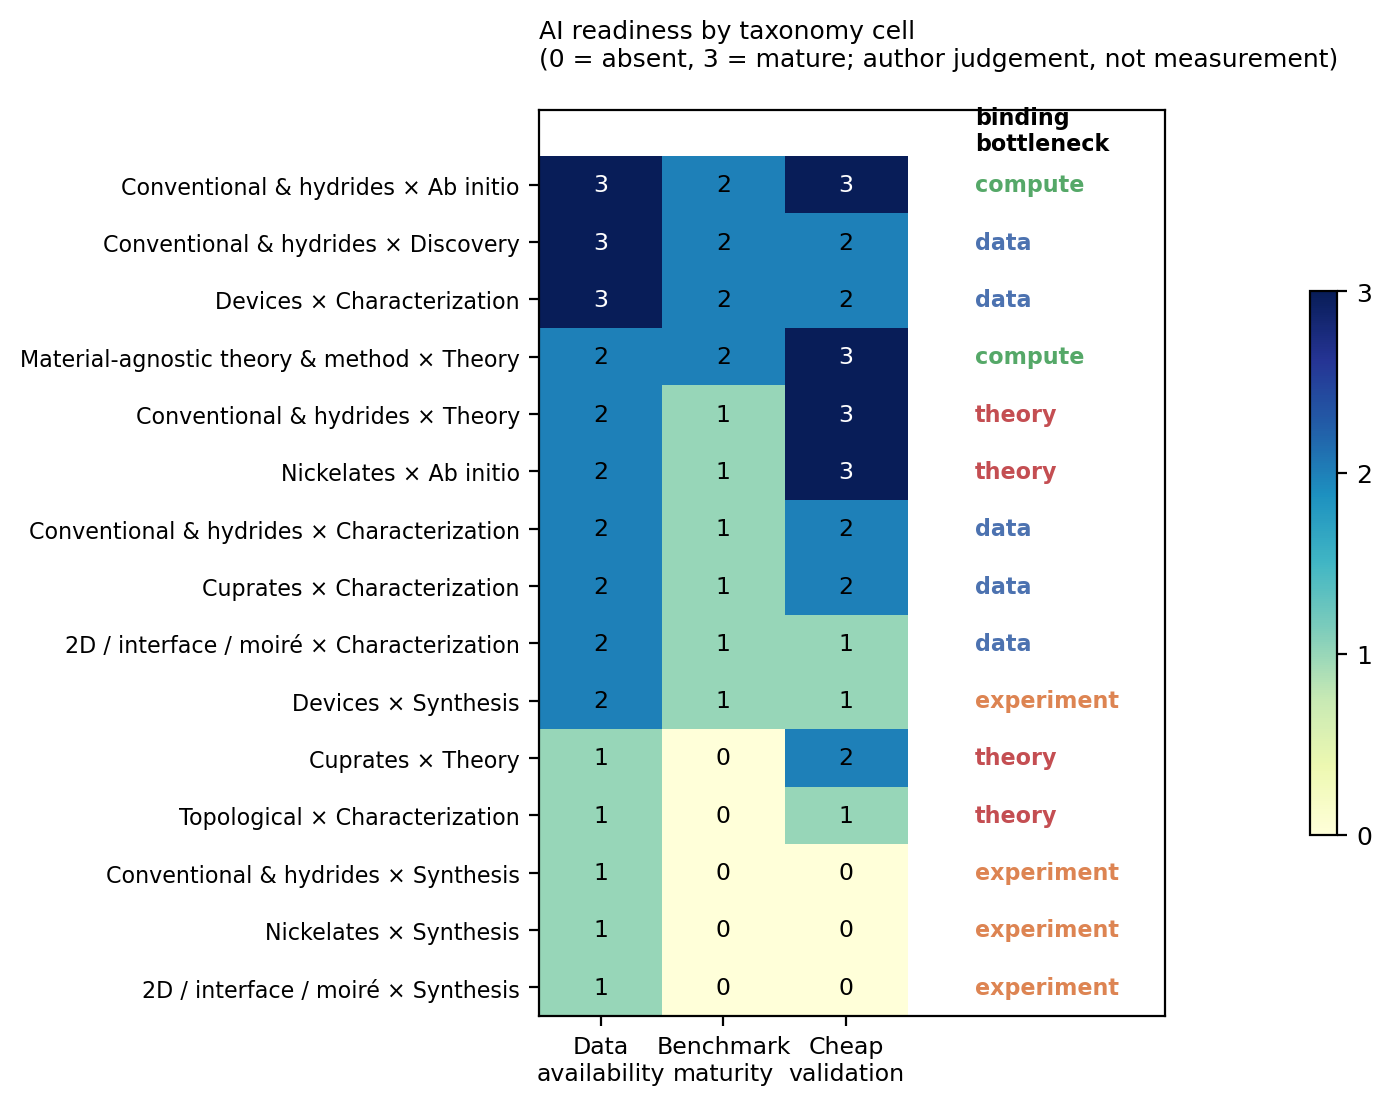
\includegraphics[keepaspectratio,alt={Figure 5: AI readiness by taxonomy cell. Scores are the author's judgement on a 0-3 scale, not measurements; the appendix states the reasoning for each cell.}]{figures/fig5_ai_readiness.png}}
\caption*{Figure 5: AI readiness by taxonomy cell. Scores are the
author's judgement on a 0-3 scale, not measurements; the appendix states
the reasoning for each cell.}
\end{figure}

\section{The three regimes}\label{the-three-regimes}

Read down Figure 5 and the cells sort into three groups.

\textbf{Cheap-validation cells, where progress is fastest and already
visible.} Conventional and hydride ab initio work scores highest: the
data exists in the form of hundreds of thousands of electron-phonon
calculations, an accepted target quantity exists in the Eliashberg
\(T_c\), and a prediction can be checked by running the calculation the
model was trained to approximate. Material-agnostic theory sits
alongside it: a neural quantum state's variational energy is checkable
against other methods on the same Hamiltonian. Both cells are
compute-limited rather than data-limited, and both are where the corpus
already shows the most AI activity. This is not a coincidence, and it is
the single strongest regularity in the survey: \textbf{machine learning
has penetrated exactly those cells where a machine can grade its own
homework.}

\textbf{Data-limited cells, where the obstacle is that measurements are
not in a usable form.} Characterization across cuprates, hydrides,
two-dimensional systems and devices falls here. The raw material is
abundant -- decades of ARPES, scanning tunnelling, transport and neutron
data -- but it lives in figures inside PDFs, in per-group formats, and
in supplementary files without schemas. The one recent large-scale
attempt to fix this for superconductivity extracted 78,203 records with
a language-model workflow \citep{itani2025large}, which is both an
encouraging result and a measure of how absent such resources were.
Device characterization scores best in this group because qubit and
detector metrology already produces standardised, high-volume,
machine-generated data, which is why the working applications in Section
5 cluster there.

\textbf{Experiment-limited cells, where nothing else is the bottleneck.}
Every synthesis cell scores 1, 0, 0. There is no shared dataset of
attempted syntheses with their outcomes, no benchmark, and validation
requires making the material. The corpus carries the corresponding
signature: one AI-tagged synthesis paper in 10,249 records. This is
where the general AI-for-materials programme has invested most visibly,
in autonomous laboratories \citep{szymanski2023autonomous}, and where
the criticism has been sharpest \citep{leeman2024challenges}.
Superconductivity makes the problem harder than the oxide-powder case
those systems target: nickelate films require topotactic reduction,
hydrides require diamond anvil cells at hundreds of gigapascals, and
moiré devices require stacking with angular precision. None of these is
a pipetting robot's problem.

\section{Where the theory bottleneck
sits}\label{where-the-theory-bottleneck-sits}

Two cells are labelled theory-limited, and the label means something
specific: additional data would not help, because there is no target
quantity a model could learn to predict. Cuprate theory is the canonical
case. Four decades of data have not produced an agreed mechanism, so
there is no equivalent of the Eliashberg function to regress against.
Nickelate ab initio work has the opposite problem in the same family:
the calculations are tractable and increasingly standard, but which
calculated quantity predicts \(T_c\) in a multi-orbital correlated
system is exactly what is unsettled.

Machine learning can still contribute in these cells, and the corpus
shows how: not by predicting \(T_c\) but by solving the models
themselves. Neural quantum states applied to the \(t\)-\(J\) and Hubbard
models \citep{lange2024simulating, rende2026superconductivity} address
the theory bottleneck directly, because the obstacle there is the cost
of solving a well-posed problem rather than the absence of a label.

\section{What the ranking implies}\label{what-the-ranking-implies}

Ordering the cells by summed score produces a priority list, and it is
not the list the field's activity implies. The highest-scoring
opportunities are ab initio screening, device characterization and
material-agnostic theory -- two of which are barely discussed in the
machine-learning-for-superconductors literature, which concentrates
instead on composition-to-\(T_c\) regression. The lowest-scoring are the
synthesis cells, which is where AI-for-materials rhetoric concentrates
most heavily.

Three consequences follow, and each is a claim that could be checked
rather than a prediction we are confident in.

\textbf{Characterization inversion is the most under-exploited
opportunity.} Spectroscopic and microscopy data is abundant, the mapping
from spectrum to physical parameter is well-posed, and validation is
cheap because independent measurements of the same sample exist. What is
missing is not method but infrastructure: standardised, openly-released,
labelled spectra. This is a dataset problem that a coordinated effort
could solve in a way that no amount of model development will.

\textbf{Synthesis will not yield to autonomous laboratories in this
field on the current design.} The binding constraint is that
superconductivity's important syntheses are extreme-condition and
low-throughput. The tractable version of the problem is narrower and
more useful: predicting whether a computationally proposed compound can
be made at all. The screening literature already generates this need --
one study noted that most of its promising ambient-pressure hydrides sit
slightly off the convex hull \citep{cerqueira2024searching} -- and a
synthesizability model trained on attempted syntheses, including the
failures, would be worth more to that pipeline than another increment of
\(T_c\)-regression accuracy.

\textbf{The field needs a held-out benchmark with experimental
resolution.} No cell in Figure 5 scores 3 on benchmark maturity. The
screening papers cannot be compared against each other, because each
reports its own candidate list validated by its own calculations. A
benchmark built from post-2024 experimentally confirmed superconductors,
with predictions time-stamped before confirmation, would separate
methods that generalise from methods that interpolate their training
set. The retraction record
\citep{snider2020retracted, dasenbrock2023retracted} makes the label
quality problem acute, and therefore makes the benchmark more valuable,
not less.

\section{Assessment}\label{assessment-3}

The pattern across Figure 5 is that AI adoption in this field tracks
validation cost far more closely than it tracks either data volume or
scientific importance. Where a calculation can check a prediction,
methods have arrived. Where an experiment is needed, they have not,
regardless of how much has been written about the cell. If that reading
is right, the highest-leverage interventions are the unglamorous ones:
release labelled characterization data, build a time-stamped benchmark,
and model synthesizability rather than synthesis.

\section{Outlook: a route to the grail, and what it
requires}\label{outlook-a-route-to-the-grail-and-what-it-requires}

The preceding sections are deliberately deflationary. This one is not,
but it earns its optimism by being specific about what would have to be
built.

The target is easy to state and has been stated for a century: a
superconductor that works at room temperature and ambient pressure, in a
material that can be made in quantity. Every partial success so far has
failed one of those three conditions. Cuprates and nickelates reach high
temperatures but not room temperature. Hydrides reach near-room
temperature but only under megabar pressure, and the claims that went
further were retracted
\citep{snider2020retracted, dasenbrock2023retracted}. Nothing in the AI
literature surveyed in Section 5 has moved any of the three constraints.

We take one recent industrial development as \emph{framing} rather than
as evidence, and say so explicitly: Anthropic's preview of a Model
Hardware Standard, a shared specification through which AI agents drive
laboratory instruments directly \citep{anthropic2026mhs}. It is a
product announcement, not a peer-reviewed result, and we cite it for
what it signals about where infrastructure is heading rather than for
any claim about superconductivity. What it signals matters here, because
Section 6 identified the instrument interface as the binding constraint
in every experiment-limited cell.

\section{Why the missing piece is the instrument interface, not the
model}\label{why-the-missing-piece-is-the-instrument-interface-not-the-model}

The argument of this survey has been that AI penetrated
superconductivity exactly where a machine could grade its own work, and
stopped where a physical experiment was required. That boundary is not a
statement about model capability. It is a statement about what a model
is connected to.

Three developments now bear on that boundary simultaneously.
Autonomous-laboratory software has matured from bespoke scripts toward
operating systems with typed, stateful device abstractions
\citep{gao2025unilabos}, and the field now frames its next phase around
six properties -- interoperable, collaborative, generalizable,
orchestrated, safe and creative -- rather than around isolated robotic
cells \citep{lee2026toward}. Multi-agent orchestration of laboratory
resources is being studied as a management problem in its own right
\citep{kusne2026managing}. And hardware-standardisation efforts aim to
collapse instrument integration from weeks to hours
\citep{anthropic2026mhs}.

If these hold, the practical consequence for superconductivity is narrow
and important: the cost of \emph{one experimental iteration} falls, and
with it the cost of the validation step that Figure 5 identifies as the
binding constraint in every synthesis cell. Nothing about that requires
a better \(T_c\) regressor.

\section{Four things that would have to be
built}\label{four-things-that-would-have-to-be-built}

\textbf{A synthesizability model trained on failures.} Section 4
established that the negative half of the synthesis record does not
exist: papers report the attempts that worked. The screening literature
has already generated the demand -- candidate lists in the hundreds,
with thermodynamic stability as the only filter, and a known caveat that
promising compounds often sit slightly off the convex hull
\citep{cerqueira2024searching}. A registry of attempted syntheses with
conditions and outcomes, failures included, is a coordination problem
rather than a research problem, and it is the single highest-leverage
dataset this survey can identify. Autonomous platforms are attractive
here for a reason usually left implicit: \textbf{a robot has no
incentive to withhold a failed run.} Instrumented synthesis generates
the negative data that human publication practice systematically
destroys.

\textbf{Instrumented characterization as a first-class output.} The same
argument applies one step downstream. Section 6 ranked characterization
inversion as the most under-exploited opportunity in the field, blocked
by data format rather than by method. An instrument operating under a
machine interface emits arrays with acquisition parameters attached by
construction. The dataset problem and the automation problem have the
same solution, and the automation is being built for other reasons.

\textbf{Extreme-condition autonomy, which is the hard case.}
Superconductivity's important syntheses are not pipetting. They are
diamond anvil cells at 200 GPa, topotactic reduction with calcium
hydride, molecular-beam epitaxy under strain, and mechanical stacking
with angular precision. Existing autonomous platforms target bulk oxide
powders, and even there the claims have been contested
\citep{leeman2024challenges}. The honest statement is that no current
self-driving laboratory addresses the syntheses this field actually
needs, and that closing that gap is an instrumentation programme
measured in years. The diamond-anvil-cell case is the one worth
attacking first: the sample is tiny, the measurement is electrical, the
parameter space is low-dimensional, and the iteration is currently gated
almost entirely by human attention.

\textbf{A benchmark with experimental resolution.} The AI-for-science
field has begun building serious evaluations -- agent suites over
research tasks \citep{bragg2025astabench}, physics-specific research
benchmarks \citep{miao2026prlbench}, reproduction of Nature-family
results \citep{wang2026naturebench}, and particle-physics analysis
reproduction \citep{faroughy2026colliderbench}. Superconductivity has
none. The version this field needs is specific: a time-stamped registry
in which candidate materials are predicted before synthesis, and scored
against what is subsequently made and measured. Only such a benchmark
can distinguish a method that generalises from one that interpolates its
training set, and its absence is why no cell in Figure 5 scores full
marks on benchmark maturity.

\section{What would falsify the
optimism}\label{what-would-falsify-the-optimism}

A position paper argues that agentic AI systems, whatever their
capabilities as co-scientists, are not built for autonomous discovery --
problem selection is distorted by what is measurable, and the loop from
hypothesis to validated result is not closed by adding autonomy
\citep{bisht2026agentic}. This survey's corpus is consistent with that
argument rather than against it, and the failure mode it predicts is
specific enough to watch for.

If the optimistic route is wrong, it will look like this: instrument
standardisation arrives, throughput rises, and the field produces more
measurements of the compounds it was already going to measure, while the
candidate lists generated by screening remain unsynthesised because the
syntheses that matter stay bespoke. Cheap iteration would then have
accelerated the cells that were never the bottleneck. The early
indicator is measurable in this survey's own terms: if the AI-tagged
synthesis count stays near one while AI-tagged characterization grows,
automation has been absorbed by the mode that was already tractable.

The complementary risk is that the loop closes on the wrong targets. The
one clearly closed prediction-synthesis-measurement loop in this
literature delivered superconductors between 2.5 and 6.5 K
\citep{li2026agentic}. A faster loop that stays in that temperature
range would be a genuine engineering achievement and no progress at all
toward the grail, because the constraint at high \(T_c\) is not
iteration speed but the absence of a theory that says where to look in
the correlated families.

\section{The honest statement of the
route}\label{the-honest-statement-of-the-route}

Putting Sections 4 through 7 together, the route this survey supports is
not ``apply a generative model to composition space.'' It is a sequence
in which each step unblocks the next:

\begin{enumerate}
\def\labelenumi{\arabic{enumi}.}
\tightlist
\item
  \textbf{Instrument the experiments}, because that produces the
  negative data and the machine-readable characterization records that
  nothing else will.
\item
  \textbf{Build the benchmark}, because without time-stamped
  experimental resolution the screening literature cannot be compared
  and therefore cannot improve.
\item
  \textbf{Model synthesizability}, because that is the tractable form of
  the bottleneck and it converts screening output into experimental
  input.
\item
  \textbf{Attack the theory bottleneck where it is well-posed}, meaning
  neural quantum states on the correlated models
  \citep{lange2024simulating, rende2026superconductivity}, because in
  cuprates and nickelates the missing thing is a solved model, not a
  larger dataset.
\end{enumerate}

Room-temperature ambient-pressure superconductivity may or may not be
reachable; that is a question about nature. What this survey can say is
that the field's current allocation of AI effort is not aimed at the
steps above, that the steps are buildable with infrastructure now
emerging, and that the first three of them are dataset and standards
problems rather than modelling problems. That is an unglamorous
conclusion, and it is the one the evidence supports.

\section{Discussion}\label{discussion}

\section{Reading the corpus's own
shape}\label{reading-the-corpuss-own-shape}

Before interpreting any proportion in this survey, three sampling facts
have to be stated, because each of them shapes the numbers.

First, the seed is a category harvest, not a topic harvest. A paper
appears because its authors chose \texttt{cond-mat.supr-con}, so the
corpus measures what the community files under superconductivity, which
is not identical to what is about superconductivity. The measured
off-topic rate within the seed is 2.5\%.

Second, the supplement is recency-biased by construction and is excluded
from every trend statement and from Table 1's grid.

Third, labels come from a model pass with 85.6\% family and 88.4\% mode
agreement against a single annotator's hand labels, and the two smallest
modes -- synthesis at 64\% recall and discovery at 54\% -- are the least
reliable. Any statement below that depends on those two counts is stated
as a hypothesis.

With those caveats, three features of the corpus seem worth explaining.

\section{Three hypotheses about the field's
shape}\label{three-hypotheses-about-the-fields-shape}

\textbf{The verifiability gradient.} AI methods appear in this corpus
almost exactly where a prediction can be checked without an experiment.
Ab initio screening, where a DFT calculation grades the model, and
neural quantum states, where a variational energy does, are the two
populated cells; synthesis, where only a furnace can settle the
question, has one paper. The hypothesis is that adoption is governed by
validation cost rather than by data volume or scientific payoff. It is
testable: if it holds, the next AI methods to arrive in this field
should show up in characterization inversion tasks, where an independent
measurement provides the check, before they show up anywhere in
synthesis.

\textbf{The label-quality trap at the top of the range.} A \(T_c\) model
is most valuable where \(T_c\) is highest, and that is precisely where
this field's experimental record is least reliable -- two retracted
room-temperature claims
\citep{snider2020retracted, dasenbrock2023retracted}, an unreplicated
ambient-pressure claim \citep{lee2023lk99}, and continuing
methodological dispute about what constitutes proof under megabar
pressure \citep{tallon2024flux}. The hypothesis is that supervised
models in this domain inherit a systematically noisier label
distribution in exactly the region they are asked to extrapolate into.
This too is testable: a model trained with and without the contested
high-\(T_c\) entries should differ measurably in its top-ranked
candidates.

\textbf{Institutional role assignment.} The AI-tagged work in this
corpus is concentrated in the material-agnostic and device families
rather than in the correlated-material families, and its authors are
frequently from computational or machine-learning-methods groups rather
than from the synthesis and spectroscopy groups whose data the methods
would need. The hypothesis is that the field's AI adoption is limited
less by method availability than by the absence of overlap between the
people who hold the data and the people who build the models. The
prediction is that the fastest progress will come from instrument groups
adopting methods internally -- which is what the qubit-readout
literature already looks like -- rather than from methods groups
acquiring physics data.

None of these is established by this survey. They are the explanations
most consistent with the corpus's shape, offered so that they can be
argued with.

\section{What would change the
assessment}\label{what-would-change-the-assessment}

Three developments would substantially revise Section 6's conclusions,
and it is worth naming them in advance.

A public, standardised corpus of labelled characterization data -- ARPES
cuts, STM maps, diffraction patterns with acquisition metadata -- would
move several cells from data-limited to method-limited in one step, and
would be the single highest-value intervention identified here.

A registry of attempted syntheses including failures would make
synthesizability prediction trainable, which is the tractable form of
the synthesis problem.

A time-stamped benchmark of experimentally confirmed superconductors,
with model predictions recorded before confirmation, would let the
screening literature be compared rather than merely accumulated. Its
absence is why no cell in Figure 5 scores 3 on benchmark maturity.

\section{Limitations of this
survey}\label{limitations-of-this-survey}

The corpus is arXiv-only and therefore under-represents applied
superconductivity published through IEEE venues and industrial device
work that is never posted. The window opens in September 2021, so
pre-window developments enter only through hand-verified anchor
citations. Labels are single-valued where the underlying reality is
often multi-valued. The AI-readiness scores in Figure 5 are the author's
judgement on a coarse scale, informed by the corpus but not derived from
it, and the appendix states the reasoning for each cell so that
individual scores can be contested. All hand labels were produced by one
annotator, so the agreement figures quoted throughout measure
consistency between one human pass and one model pass, not accuracy
against an external standard.

\section{Conclusion}\label{conclusion}

This survey mapped five years of superconductivity research -- 10,249
arXiv preprints after off-topic filtering -- onto two axes, material
family and mode of inquiry, and then asked of each cell what a
machine-learning method could contribute there.

The mapping produced three findings. Machine learning has barely entered
this field: 1.2\% of the systematically harvested seed uses an AI method
in its own work. Where it has entered, it clusters where predictions can
be checked by calculation rather than by experiment -- ab initio
screening and neural quantum states -- and in device metrology, where
instruments generate their own labelled data. And the field's actual
bottleneck, synthesis, is the cell with the least usable data and the
fewest methods: one AI-tagged paper in the entire corpus.

The gap between what the screening literature predicts and what has been
made and measured is the survey's most concrete result. Recent screens
report candidates above 200 K; the one clearly closed
prediction-synthesis-measurement loop in the recent literature delivered
superconductors between 2.5 and 6.5 K \citep{li2026agentic}. Both facts
are real, and holding them together is the correct posture toward AI for
superconductivity.

For anyone deciding where to apply AI for Science effort in this field,
the ranking that follows from Figure 5 is: release labelled
characterization data and build inversion models against it; construct a
time-stamped benchmark so screening methods can be compared; and model
synthesizability rather than attempting to automate synthesis. These are
less exciting than inverse-designing a room-temperature superconductor,
and they are what the structure of the field currently supports.

Section 7 argues that the first two of these are becoming buildable for
reasons outside this field: laboratory hardware is being standardised
for machine operation, and an instrumented experiment emits the negative
results and the machine-readable spectra that human publication practice
does not. That makes the instrument interface, rather than model
capability, the variable most likely to move this assessment. It also
sets the test: if throughput rises while the AI-tagged synthesis count
stays near one, automation will have accelerated the modes that were
never the bottleneck.

\section{Data availability}\label{data-availability}

The corpus, labels, prompts, hand-labelled validation sets and all
scripts are released at
\url{https://github.com/deepgrounding/superconductivity-ai-survey}. The
repository contains the frozen seed harvest (\texttt{sc\_seed.csv}), the
canonical labelled corpus (\texttt{sc\_corpus\_v1.csv}), the raw
per-month arXiv responses that reproduce the harvest, the language-model
label cache (\texttt{llm\_labels.jsonl}), the two hand-labelled
validation sets (\texttt{label\_truth.csv},
\texttt{ai\_label\_truth.csv}), and the harvesting, labelling, figure
and build scripts. Bibliography entries for corpus papers are generated
from the corpus; anchor references outside the harvest window are
hand-verified against Crossref and kept separately.

\section{Appendix: reasoning behind the AI-readiness
scores}\label{appendix-reasoning-behind-the-ai-readiness-scores}

Figure 5 scores each discussed cell on data availability, benchmark
maturity and cheap validation, on a 0-3 scale, and names the binding
bottleneck. The scores are the author's judgement. This appendix states
the reasoning so that individual cells can be contested; the scoring
table itself is in \texttt{build\_concept\_figures.py}, so a reader who
disagrees can change a row and regenerate the figure.

{\def\LTcaptype{none} % do not increment counter
\begin{longtable}[]{@{}
  >{\raggedright\arraybackslash}p{(\linewidth - 2\tabcolsep) * \real{0.5000}}
  >{\raggedright\arraybackslash}p{(\linewidth - 2\tabcolsep) * \real{0.5000}}@{}}
\toprule\noalign{}
\begin{minipage}[b]{\linewidth}\raggedright
Cell
\end{minipage} & \begin{minipage}[b]{\linewidth}\raggedright
Reasoning
\end{minipage} \\
\midrule\noalign{}
\endhead
\bottomrule\noalign{}
\endlastfoot
Conventional × ab initio & Data 3: hundreds of thousands of
electron-phonon calculations exist, \textasciitilde7,000 of them
assembled as a single training set \citep{cerqueira2023sampling}.
Benchmark 2: the Eliashberg \(T_c\) is an accepted target, but no shared
held-out set. Validation 3: a DFPT calculation settles it. Bottleneck
compute. \\
Conventional × discovery & Data 3 for composition-\(T_c\) pairs.
Benchmark 2. Validation 2: cheap computationally, expensive
experimentally, and the screening literature stops at the computational
step. Bottleneck data, specifically the absence of negative results and
of verified high-\(T_c\) labels. \\
Conventional × synthesis & Data 1: recipes in prose, successes only.
Benchmark 0. Validation 0: diamond anvil cell at megabar pressures.
Bottleneck experiment. \\
Conventional × characterization & Data 2, benchmark 1, validation 2.
High-pressure measurement is hard but the quantities are conventional.
Bottleneck data. \\
Conventional × theory & Data 2, benchmark 1, validation 3:
Migdal-Eliashberg is a well-posed calculation. Bottleneck theory, in the
narrow sense that anharmonicity and quantum ionic effects are where the
physics is unsettled. \\
Cuprate × theory & Data 1, benchmark 0, validation 2. Four decades of
data with no agreed target quantity to regress against. Bottleneck
theory. \\
Cuprate × characterization & Data 2: abundant spectra, almost none
machine-readable. Benchmark 1, validation 2. Bottleneck data. \\
Nickelate × ab initio & Data 2, benchmark 1, validation 3: the
calculations are tractable and increasingly standard. Bottleneck theory:
which computed quantity predicts \(T_c\) in a multi-orbital correlated
system is exactly what is unsettled. \\
Nickelate × synthesis & Data 1, benchmark 0, validation 0. Topotactic
reduction and strained epitaxy, with oxygen stoichiometry as the
decisive and poorly recorded variable \citep{zhou2023investigations}.
Bottleneck experiment. \\
2D / interface × characterization & Data 2: gate-tunable transport is
parameterised and dense. Benchmark 1. Validation 1: each stack is
unique, so re-measurement is not free. Bottleneck data. \\
2D / interface × synthesis & Data 1, benchmark 0, validation 0.
Mechanical stacking with angular precision. Bottleneck experiment. \\
Topological × characterization & Data 1, benchmark 0, validation 1. The
disagreement is about what a measurement means, so a label is not well
defined. Bottleneck theory. \\
Device × characterization & Data 3: qubit and detector metrology is
machine-generated, standardised and high-volume. Benchmark 2. Validation
2. Bottleneck data, and the highest-scoring measurement cell in the
survey. \\
Device × synthesis & Data 2: fabrication process data exists in
industrial settings, mostly unpublished. Benchmark 1, validation 1.
Bottleneck experiment. \\
Material-agnostic × theory & Data 2, benchmark 2, validation 3: a
variational energy is comparable against other methods on the same
Hamiltonian. Bottleneck compute. \\
\end{longtable}
}

\bibliography{references}

\end{document}
